% !TEX program = xelatex
% =====================================================================
% ScoutAgent 期末报告 final_report.tex
%
% 编译说明：
%   1. 使用 XeLaTeX 编译（命令：xelatex final_report.tex）。
%   2. 本报告仅引用以下外部图片，统一存放于同目录 media/ 下：
%        - media/dhu.png            封面校徽
%        - media/enterprise.png     第 5 章 企业与岗位工作台截图
%        - media/candidate.png      第 5 章 候选人库截图
%        - media/dashboard.png      第 5 章 评估看板截图
%        - media/assistant.png      第 5 章 深度评估 Agent 截图
%        - media/eval.png           第 5 章 Eval 系统截图
%      其余所有架构图、流程图、ER 图、拓扑图均由 TikZ 直接绘制，
%      无需任何额外资源。
%   3. 若 media/ 中暂缺图片，可临时将对应 \includegraphics 行注释掉，
%      或将文件替换为任意同名 PNG，即可顺利编译。
% =====================================================================
\documentclass[12pt,a4paper]{ctexart}

% ======================
% Packages
% ======================
\usepackage{geometry}
\usepackage{graphicx}
\usepackage{xcolor}
\usepackage{amsmath, amssymb}
\usepackage{array}
\usepackage{booktabs}
\usepackage{tabularx}
\usepackage{setspace}
\usepackage{titlesec}
\usepackage{fancyhdr}
\usepackage{float}
\usepackage{tikz}
\usetikzlibrary{positioning,arrows.meta,shapes.geometric,shapes.symbols,fit,backgrounds,calc}
\usepackage{tcolorbox}
\tcbuselibrary{listings, breakable}
\usepackage{enumitem}
\newcolumntype{L}[1]{>{\raggedright\arraybackslash}p{#1}}
\newcolumntype{C}[1]{>{\centering\arraybackslash}p{#1}}
\newcolumntype{R}[1]{>{\raggedleft\arraybackslash}p{#1}}

\usepackage[colorlinks=true, linkcolor=black, citecolor=green, urlcolor=cyan]{hyperref}

% ======================
% 页面设置
% ======================
\geometry{a4paper,left=2.5cm,right=2.5cm,top=2.5cm,bottom=2.5cm}
\setlength{\headheight}{15pt}
\setstretch{1.3}

% ======================
% 中英混排断行：避免英文 / typewriter 长串撑出右边距
% ======================
\setlength{\emergencystretch}{3em}
\tolerance=2000
\hbadness=2000
% 提供一个允许在任意位置断行的等宽命令 \tk{...}，用于路径、API 名等长字符串
% 用法：\tk{redis/redis-stack-server:latest} 替代 \texttt{redis/redis-stack-server:latest}
\usepackage{seqsplit}
\newcommand{\tk}[1]{\texttt{\seqsplit{#1}}}

% ======================
% 颜色
% ======================
\definecolor{titleblue}{RGB}{65,105,225}
\definecolor{darkgreen}{RGB}{0,120,70}
\definecolor{highlight}{RGB}{200,30,30}

% ======================
% 标题样式
% ======================
\titleformat{\section}
{\Large\bfseries\color{titleblue}}
{\thesection}{1em}{}

\titleformat{\subsection}
{\large\bfseries\color{darkgreen}}
{\thesubsection}{1em}{}

% ======================
% 页眉页脚
% ======================
\pagestyle{fancy}
\fancyhf{}
\fancyhead[L]{ScoutAgent Project}
\fancyhead[R]{智能技术工程实训}
\fancyfoot[C]{\thepage}

\begin{document}

% ==================================================
% 封面
% ==================================================
\begin{titlepage}
\thispagestyle{empty}
\centering

\vspace*{0.6cm}


\includegraphics[width=0.62\textwidth]{media/dhu.png}

\vspace{1.2cm}

{\Huge\bfseries\color{titleblue}人工智能应用实践系统实现报告}

\vspace{0.6cm}

{\LARGE\bfseries 面向招聘场景的智能人才评估与推荐平台}

\vspace{0.3cm}

{\large ScoutAgent：基于 LangGraph 的多智能体协作系统}

\vspace{1.4cm}

\begin{minipage}{0.75\textwidth}
\renewcommand{\arraystretch}{1.9}
\begin{tabular}{>{\bfseries\large}l >{\large}l}
组\quad 员： & 郑吴穷 \quad 于笑 \quad 李汉尧 \\
学\quad 号： & 231380128 \quad 231380124 \quad 220820114 \\
学\quad 院： & 信息与智能科学学院 \\
专\quad 业： & 智能科学与技术 \\
课程名称： & 智能技术工程实训 \\
报告类型： & 系统实现报告 \\
日\quad 期： & 2026/4/20 \\
\end{tabular}
\end{minipage}

\vfill

{\large 东华大学}

\vspace{0.2cm}

{\large 信息与智能科学学院}

\vspace{0.4cm}

\end{titlepage}

% ==================================================
% 摘要
% ==================================================
\thispagestyle{empty}
\begin{center}
{\Large\bfseries\color{titleblue}摘\quad 要}
\end{center}

\begin{spacing}{1.4}
\noindent
当前互联网招聘场景普遍存在四类难以回避的痛点：基于关键词的简历筛选无法刻画真实技能匹配、候选人对简历的过度包装难以察觉、技术能力评估缺乏可量化的过程指标、多轮评估信息散落且难以沉淀为组织资产。本文以\textbf{ScoutAgent}——一个面向技术招聘场景的多智能体协作评估平台为对象，给出从行业痛点到工程落地的完整方案。系统以 \textbf{LangGraph} 为编排核心，对外暴露 \textbf{ReAct} 与 \textbf{Plan-and-Execute} 两套图，统一组合 \textbf{Tools / Skills / MCP} 三层工具体系；在记忆侧采用 \textbf{Redis Checkpointer} 维护工作记忆、\textbf{PostgreSQL} 持久化企业级与岗位级偏好；在算法侧落地了三项关键技术：基于通义千问与思维链的结构化抽取（F1 由 66\% 提升至 78\%）、基于 \textbf{Neo4j} 的技术知识图谱与 \textbf{GraphRAG} 匹配增强（JD-CV 二分类准确率由 74.3\% 提升至 85.2\%），以及面向简历过度包装检测的 \textbf{SFT+DPO} 两阶段对齐（Pairwise Accuracy 由 73.5\% 提升至 88.5\%）。系统采用 React + FastAPI + 三类存储 + Docker Compose 的工程拓扑，已在阿里云 ECS 与 AutoDL GPU 之间通过 SSH 端口转发完成端到端联调。本报告分五章依次呈现选题背景与需求、Agent 架构设计、关键算法与实验验证、技术栈与部署、以及前端系统功能展示。

\vspace{0.8cm}

\noindent\textbf{关键词}：LLM Agent；LangGraph；GraphRAG；知识图谱；SFT；DPO；招聘评估
\end{spacing}

\newpage

% ==================================================
% 目录
% ==================================================
\setcounter{tocdepth}{2}
\tableofcontents
\newpage

% ==================================================
% 第一章 选题背景与需求分析
% ==================================================
\section{选题背景与需求分析}\label{sec:bg}

\subsection{招聘场景的核心矛盾}

招聘是一个\textbf{信息密度高、判断成本重、容错率低}的典型业务场景：岗位描述（JD）通常以结构化的硬性要求与软性偏好呈现，而候选人简历（CV）却是高度个性化的非结构化叙述。HR 每天的工作，本质上就是在大量异构文本之间寻找匹配、辨别真伪、给出综合判断——这正是大语言模型最适合发挥的场景。然而，当前主流的 ATS（Applicant Tracking System）仍以关键词过滤为主，距离"理解候选人"还有相当差距。

ScoutAgent 的选题正是从这一矛盾出发：把 HR 工作中"最重复、最易错、最难沉淀"的环节交给 Agent，让人回到真正需要判断的位置。

\subsection{招聘流程中的四类核心痛点}

我们将企业实际招聘流程拆解为初筛、深筛、技评、终评四个阶段，分析每个阶段 HR 实际承担的工作以及对应的痛点（见表~\ref{tab:hr-pain-stage}）。

\begin{table}[H]
\centering
\renewcommand{\arraystretch}{1.35}
\caption{招聘流程各阶段的 HR 实际工作与主要痛点}
\label{tab:hr-pain-stage}
\begin{tabular}{L{1.6cm} L{4.6cm} L{6.0cm}}
\toprule
\textbf{阶段} & \textbf{HR 实际承担的工作} & \textbf{主要痛点} \\
\midrule
初筛 & 关键词搜索简历池 & 同义词、上下位关系、技术栈迁移识别能力差 \\
深筛 & 阅读项目经历与经历叙述 & 包装、虚标、年限注水难以辨别 \\
技评 & 出题、阅卷、看代码 & 题目同质化、判分主观、无法考察过程 \\
终评 & 多轮拍板、形成结论 & 信息散落多处，难以复盘与沉淀经验 \\
\bottomrule
\end{tabular}
\end{table}

四个阶段的痛点不是孤立存在，而是从前到后串成一条流水线（见图~\ref{fig:pain-pipeline}）。每一处痛点都会在下一阶段被放大：初筛把人选错了，深筛就要花更多时间补救；深筛没识破包装，技评和终评就只能在错误的样本池里挑选。

\begin{figure}[H]
\centering
\begin{tikzpicture}[
  font=\small, >=Stealth,
  pool/.style={draw, rounded corners=4pt, fill=blue!8,
               minimum width=3.6cm, minimum height=0.85cm, align=center},
  pain/.style={draw, rounded corners=4pt, fill=red!10,
               minimum width=3.4cm, minimum height=0.95cm, align=center},
  result/.style={draw, rounded corners=4pt, fill=green!10,
              minimum width=3.6cm, minimum height=0.85cm, align=center},
  arr/.style={->, thick, color=gray!65},
]
\node[pool]   (pool) at (0,0) {简历池\\每岗位 100$\sim$1000 份};
\node[pain]   (p1) at (0,-1.6)  {痛点 1：JD-CV 匹配低效\\关键词 $\neq$ 能力};
\node[pain]   (p2) at (0,-3.0)  {痛点 2：简历真实性存疑\\包装产业化};
\node[pain]   (p3) at (0,-4.4)  {痛点 3：技术能力难量化\\题海与直觉};
\node[pain]   (p4) at (0,-5.8)  {痛点 4：多轮评估碎片化\\经验难沉淀};
\node[result] (decision) at (0,-7.4) {最终录用决策};

\draw[arr] (pool) -- (p1);
\draw[arr] (p1)   -- (p2);
\draw[arr] (p2)   -- (p3);
\draw[arr] (p3)   -- (p4);
\draw[arr] (p4)   -- (decision);
\end{tikzpicture}
\caption{招聘流程中的四类核心痛点流水线}
\label{fig:pain-pipeline}
\end{figure}

\textbf{痛点一：关键词匹配 $\neq$ 能力匹配。}\quad 纯文本匹配天然处理不了"语义 + 结构"的双重对齐：技术栈存在大量\textbf{同义词}（K8s 与 Kubernetes）、\textbf{上下位关系}（Spring Cloud 属于微服务）和\textbf{迁移能力}（具备 Java 后端经验大概率能上手 Go 后端）。

\textbf{痛点二：简历"通用化包装"已成产业。}\quad 市面上充斥着"简历优化教程"，候选人往往针对 JD 反向定制简历，常见手法包括职责膨胀、技术堆砌、时间含糊与项目挪用。单点信息无法证伪，只能通过\textbf{跨字段交叉验证}才能识别。

\textbf{痛点三：技术能力评估靠"题海 + 直觉"。}\quad 传统笔试与白板题与真实工程能力相去甚远，HR 真正想知道的是候选人的解题路径、代码结构和被追问后的反应，但现有平台只能给出"通过率"，无法提供过程评估。

\textbf{痛点四：多轮评估信息"碎片化"。}\quad 初筛 Excel、面试官口头反馈、技术评分表、HR 邮件等信息散落在多个系统中，最终决策时拼不起来；HR 一旦离职，组织对该岗位的偏好积累也随之消失。

\subsection{从行业痛点到技术选型的反向推演}

针对上述四类痛点，本系统在技术选型上做了一一对应的设计（见表~\ref{tab:pain-tech}）。整体思路是：与其面向"AI 简历筛选器"做单点替代，不如面向"AI HR 助手"做\textbf{增强式协作}——把 Agent 嵌入 HR 现有的工作流，让其调用知识图谱与外部工具、记住每个客户的偏好、按计划完成多步评估，并把全过程以可追溯报告的形式沉淀下来。

\begin{table}[H]
\centering
\renewcommand{\arraystretch}{1.35}
\caption{行业痛点与技术选型的对应关系}
\label{tab:pain-tech}
\begin{tabular}{L{3.8cm} L{4.0cm} L{5.0cm}}
\toprule
\textbf{行业痛点} & \textbf{技术选型} & \textbf{核心思路} \\
\midrule
同义词 / 上下位概念 & Neo4j 知识图谱 + GraphRAG & 把"技术栈"建成图，用结构推理代替字符串匹配 \\
包装与虚标 & 真实性检测 Agent & LLM 跨"JD / CV / 项目 / 测试"四源比对 \\
能力评估粗糙 & 代码执行工具 + 过程评估 & Agent 调工具拿运行结果，结合解题过程评分 \\
决策碎片化 & Plan-and-Execute + 报告生成 & 拆解评估流程，输出结构化 Markdown 报告 \\
经验流失 & 企业级 / 岗位级偏好库 & LLM 自动识别硬性要求并 upsert 到 PG \\
\bottomrule
\end{tabular}
\end{table}

\subsection{为什么必须是 Agent，而不是单次 LLM 调用}

回到技术路线本身：在 JD 与 CV 文本上做一次 prompt 调用，让 LLM 直接给出匹配分，是否就够用？我们认为不够。招聘任务的特征决定了它必须以 Agent 形态实现：

\begin{itemize}[itemsep=3pt]
  \item 需要\textbf{外部能力}：知识图谱、代码沙箱、第三方系统等都不可能塞进 prompt，必须通过 \textbf{Function Calling} 在运行时调用；
  \item 需要\textbf{跨会话记忆}：同一家客户的招聘偏好、同一个岗位的硬性要求需要被记住，必须有 \textbf{Memory} 层；
  \item 需要\textbf{多步骤拆解}：先匹配再验真再技评再综合，需要 \textbf{Planning} 控制执行流；
  \item 需要\textbf{可解释性}：HR 必须能看到 Agent 调了哪些工具、走过哪些步骤，才能信任最终结论。
\end{itemize}

单次问答只能解决"问题"，Agent 才能解决"流程"。这正是 ScoutAgent 必须以 Agent 架构落地的根本原因，也奠定了第~\ref{sec:agent}~章的设计基调。

\subsection{选题立意与价值定位}

在产品定位上，ScoutAgent 与传统简历筛选工具有本质差异（见表~\ref{tab:position-compare}）：传统工具的目标是"提升处理速度"，本系统的目标是"提升判断质量"；传统工具输出一个分数，本系统输出一份带证据链的报告；传统工具替代 HR，本系统增强 HR。

\begin{table}[H]
\centering
\renewcommand{\arraystretch}{1.35}
\caption{ScoutAgent 与传统筛选工具的定位对比}
\label{tab:position-compare}
\begin{tabular}{L{2.4cm} L{4.6cm} L{5.4cm}}
\toprule
\textbf{维度} & \textbf{传统筛选工具} & \textbf{ScoutAgent} \\
\midrule
目标 & 提升处理速度 & 提升判断质量 \\
输出 & 一个匹配分数 & 一份带证据链的结构化报告 \\
对 HR 的关系 & 替代 / 引发被取代焦虑 & 协作式增强 \\
可解释性 & 黑盒打分 & 计划 + 工具调用全过程可见 \\
经验沉淀 & 无 & 企业级与岗位级偏好持续学习 \\
\bottomrule
\end{tabular}
\end{table}

进一步从价值闭环看，本项目同时具备技术、业务与社会三层意义：技术层面在真实业务中验证 Function Calling、Memory、Planning 三大模块的协同；业务层面把 HR 每岗位评估时间从"几小时/份"压缩到"几分钟/份"并产出可追溯报告；社会层面降低"靠包装上岗"与"靠学历过滤"的概率，让真实能力被看见，让非典型背景候选人获得更公平的机会。

% ==================================================
% 第二章 Agent 架构设计
% ==================================================
\section{Agent 架构设计}\label{sec:agent}

\subsection{整体架构总览}

ScoutAgent 后端 Agent 基于 \textbf{LangGraph} 构建，对外暴露两套并列的图：用于实时招聘对话的 \textbf{Chat Graph}（ReAct 范式）与用于复杂任务编排的 \textbf{Planning Graph}（Plan-and-Execute 范式）。两套图通过统一的工具解析层 \texttt{tool\_resolver} 在运行时动态绑定能力，并共用同一套两层记忆体系（短时工作记忆 + 长期偏好沉淀）。整体结构如图~\ref{fig:agent-overview}~所示。

\begin{figure}[H]
\centering
\begin{tikzpicture}[
  font=\small, >=Stealth,
  user/.style={draw, rounded corners=4pt, fill=blue!8, align=center,
               minimum width=2.0cm, minimum height=0.7cm},
  api/.style ={draw, rounded corners=4pt, fill=orange!12, align=center,
               minimum width=3.4cm, minimum height=0.7cm},
  graph/.style={draw, rounded corners=4pt, fill=green!9, align=center,
                minimum width=3.4cm, minimum height=0.85cm},
  res/.style={draw, rounded corners=4pt, fill=yellow!18, align=center,
              minimum width=3.0cm, minimum height=0.7cm},
  tool/.style={draw, rounded corners=3pt, fill=blue!5, align=center,
               minimum width=2.4cm, minimum height=0.65cm, font=\footnotesize},
  store/.style={draw, rounded corners=4pt, fill=purple!10, align=center,
                minimum width=2.6cm, minimum height=0.7cm, font=\footnotesize},
  arr/.style={->, thick, color=gray!60},
  darr/.style={->, dashed, thick, color=gray!55},
]
\node[user]  (u)   at (0,0)         {用户};
\node[api]   (api) at (3.6,0)       {FastAPI Router};
\node[graph] (chat) at (1.6,-1.7)   {Chat Graph\\\footnotesize ReAct};
\node[graph] (plan) at (5.6,-1.7)   {Planning Graph\\\footnotesize Plan-and-Execute};
\node[res]   (res)  at (3.6,-3.4)   {tool\_resolver};

\node[tool]  (t1) at (-0.6,-5.0) {Tools\\原生函数};
\node[tool]  (t2) at (3.6,-5.0)  {Skills\\SKILL.md};
\node[tool]  (t3) at (7.8,-5.0)  {MCP\\外部 Server};

\node[store] (rd) at (-1.4,-2.1) {Redis\\Checkpointer};
\node[store] (pg) at (8.6,-2.1)  {PostgreSQL\\偏好库};

\draw[arr] (u)  -- (api);
\draw[arr] (api) -- (chat);
\draw[arr] (api) -- (plan);
\draw[arr] (chat) -- (res);
\draw[arr] (plan) -- (res);
\draw[arr] (res) -- (t1);
\draw[arr] (res) -- (t2);
\draw[arr] (res) -- (t3);

\draw[darr] (chat.west) to[bend right=20] node[left,font=\tiny]{checkpoint} (rd.north);
\draw[darr] (plan.east) to[bend left=20]  node[right,font=\tiny]{long-term} (pg.north);
\end{tikzpicture}
\caption{ScoutAgent 后端 Agent 整体架构总览}
\label{fig:agent-overview}
\end{figure}

\subsection{Function Calling：三层工具体系}

把"可被 LLM 调用的能力"做了清晰的分层是 ScoutAgent 在 Function Calling 设计上的核心抽象：每一层职责不同，但通过统一的 \texttt{resolve\_tools(config)} 在每次推理前组装为一份扁平的工具列表，再交给 LLM 绑定。三层结构如图~\ref{fig:fc-layers}~所示，三层之间的对比见表~\ref{tab:fc-compare}。

\begin{figure}[H]
\centering
\begin{tikzpicture}[
  font=\small, >=Stealth,
  layer/.style={draw, rounded corners=5pt, dashed, fill=blue!4,
                inner sep=8pt},
  l1/.style={draw, rounded corners=3pt, fill=blue!10,
             minimum width=3.4cm, minimum height=0.6cm, align=center, font=\footnotesize},
  l2/.style={draw, rounded corners=3pt, fill=green!10,
             minimum width=3.4cm, minimum height=0.6cm, align=center, font=\footnotesize},
  l3/.style={draw, rounded corners=3pt, fill=purple!10,
             minimum width=3.4cm, minimum height=0.6cm, align=center, font=\footnotesize},
  res/.style={draw, rounded corners=4pt, fill=orange!15,
              minimum width=4.0cm, minimum height=0.85cm, align=center},
  arr/.style={->, thick, color=gray!60},
]
\node[res] (res) at (0,0) {resolve\_tools(config)\\\footnotesize 运行时按 session 装配};

\node[l1] (a1) at (-5.2,-2.0) {query\_knowledge\_graph};
\node[l1] (a2) at (-5.2,-2.85) {save\_preference\_memory};
\node[l1] (a3) at (-5.2,-3.7) {check\_resume\_authenticity};

\node[l2] (b1) at (0,-2.0)  {execute\_skill\_script};
\node[l2] (b2) at (0,-2.85) {load\_skill\_reference};

\node[l3] (c1) at (5.2,-2.0)  {pg\_server (MCP)};
\node[l3] (c2) at (5.2,-2.85) {第三方 MCP Server};

\begin{scope}[on background layer]
  \node[layer, fit=(a1)(a2)(a3), label=above:{\footnotesize\bfseries Layer 1 · Tools 原生工具}] {};
  \node[layer, fit=(b1)(b2),    label=above:{\footnotesize\bfseries Layer 2 · Skills 标准技能}] {};
  \node[layer, fit=(c1)(c2),    label=above:{\footnotesize\bfseries Layer 3 · MCP 外部协议}] {};
\end{scope}

\draw[arr] (res.south) -- ++(0,-0.5) -| (a1.north);
\draw[arr] (res.south) -- ++(0,-0.5) -| (b1.north);
\draw[arr] (res.south) -- ++(0,-0.5) -| (c1.north);
\end{tikzpicture}
\caption{Function Calling 三层工具体系}
\label{fig:fc-layers}
\end{figure}

\begin{table}[H]
\centering
\renewcommand{\arraystretch}{1.3}
\caption{Tools / Skills / MCP 三类工具对比}
\label{tab:fc-compare}
{\small
\begin{tabular}{L{1.8cm} L{3.6cm} L{3.6cm} L{3.6cm}}
\toprule
\textbf{维度} & \textbf{Tools} & \textbf{Skills} & \textbf{MCP} \\
\midrule
定位 & 业务原子能力 & 领域专家手册 + 可选脚本 & 外部进程能力 \\
载体 & Python 函数（StructuredTool） & SKILL.md 目录 & 独立进程（stdio / http / sse）\\
注册方式 & 模块导入 BASE\_TOOLS & YAML frontmatter 扫描 & mcp\_servers.json \\
发现时机 & 启动时静态导入 & 启动时扫描目录 & 启动时连接 + get\_tools() \\
典型例子 & KG 查询、保存偏好、真实性检测 & jd-cv-match、authenticity-check & Postgres MCP Server \\
\bottomrule
\end{tabular}
}
\end{table}

\subsubsection{Tools：原生函数工具}

最底层的 Tools 直接以 Python 函数 + Pydantic Schema 实现，注册路径在 \texttt{backend/app/agent/tool\_resolver.py}：

\begin{quote}\small
\texttt{BASE\_TOOLS = [query\_knowledge\_graph, save\_preference\_memory, check\_resume\_authenticity]}
\end{quote}

每个 Tool 都被封装成 \texttt{StructuredTool}，LLM 看到的只有 \texttt{name}、\texttt{description} 与 \texttt{args\_schema}，看不到具体实现，从而保证调用的安全性与可替换性。

\subsubsection{Skills：渐进披露的标准技能}

Skills 是一种"约定大于配置"的能力封装，每个 Skill 是一个目录，包含 \texttt{SKILL.md}（YAML frontmatter + 主体指令）、\texttt{references/} 与 \texttt{scripts/}。Skills 的关键设计是\textbf{渐进披露}（progressive disclosure）：始终把所有 Skill 的元数据放进 system prompt，让 LLM 知道有哪些能力存在；当用户激活后再注入完整 \texttt{SKILL.md} 主体；引用文档与脚本则按需通过工具调用加载（图~\ref{fig:skills-progressive}）。这样 system prompt 始终保持紧凑，只在确实需要时才"展开"详细内容。

\begin{figure}[H]
\centering
\begin{tikzpicture}[
  font=\small, >=Stealth,
  stepBox/.style={draw, rounded corners=4pt, fill=green!8,
               minimum width=3.0cm, minimum height=0.78cm, align=center},
  dec/.style={draw, diamond, fill=yellow!18, aspect=2.4, align=center,
              text width=2.6cm, font=\footnotesize, inner sep=1pt},
  arr/.style={->, thick, color=gray!65},
]
\node[stepBox] (s0) at (0,0) {Skill 安装\\元数据 name+desc};
\node[stepBox] (s1) at (4.6,0) {元数据进 system prompt\\$\sim$100 tokens};
\node[dec]  (d1) at (4.6,-2.0) {用户激活?};
\node[stepBox] (s2) at (10.0,-2.0) {SKILL.md 主体\\注入 system prompt};
\node[dec]  (d2) at (10.0,-4.0) {LLM 判定需要?};
\node[stepBox] (s3) at (4.6,-4.0)  {load\_skill\_reference\\加载 references/};
\node[stepBox] (s4) at (10.0,-5.6) {execute\_skill\_script\\运行 scripts/};

\draw[arr] (s0) -- (s1);
\draw[arr] (s1) -- (d1);
\draw[arr] (d1) -- node[above,font=\tiny]{是} (s2);
\draw[arr] (s2) -- (d2);
\draw[arr] (d2) -- node[above,font=\tiny]{文档} (s3);
\draw[arr] (d2) -- node[right,font=\tiny]{脚本} (s4);
\end{tikzpicture}
\caption{Skills 渐进披露的三档加载策略}
\label{fig:skills-progressive}
\end{figure}

\subsubsection{MCP：外部协议层}

MCP（Model Context Protocol）把"工具"做成独立进程，用统一协议通信，便于把数据库、第三方系统等异构能力以最小耦合的方式接入 Agent。MCP Server 的注册靠 \texttt{mcp\_servers.json} 声明式配置；启动顺序与连接流程如图~\ref{fig:mcp-seq}~所示。

\begin{figure}[H]
\centering
\begin{tikzpicture}[
  font=\small, >=Stealth,
  actor/.style={draw, rounded corners=3pt, fill=blue!10, minimum width=2.4cm,
                minimum height=0.55cm, align=center, font=\footnotesize},
  msg/.style={->, thick, color=gray!65},
]
\node[actor] (app)  at (0,0)      {FastAPI lifespan};
\node[actor] (reg)  at (3.6,0)    {MCPServerRegistry};
\node[actor] (mgr)  at (7.2,0)    {MCPClientManager};
\node[actor] (srv)  at (10.8,0)   {MCP Server 进程};

\draw[thick] (app.south) -- (0, -5.6);
\draw[thick] (reg.south) -- (3.6,-5.6);
\draw[thick] (mgr.south) -- (7.2,-5.6);
\draw[thick] (srv.south) -- (10.8,-5.6);

\draw[msg] (0,-0.7)  -- node[above,font=\tiny]{discover(json)} (3.6,-0.7);
\draw[msg] (3.6,-1.4) -- ++(1.5,0) -- ++(0,-0.05) -- ++(-1.5,0);
\node[font=\tiny, anchor=west] at (3.7,-1.4) {Pydantic 校验 + 默认值合并};

\draw[msg] (0,-2.1)  -- node[above,font=\tiny]{init(registry)} (7.2,-2.1);
\draw[msg] (7.2,-2.8) -- node[above,font=\tiny]{建立连接} (10.8,-2.8);
\draw[msg] (7.2,-3.5) -- node[above,font=\tiny]{get\_tools()} (10.8,-3.5);
\draw[msg] (10.8,-4.2) -- node[above,font=\tiny]{BaseTool[] + schema} (7.2,-4.2);
\draw[msg] (7.2,-4.9) -- ++(1.5,0) -- ++(0,-0.05) -- ++(-1.5,0);
\node[font=\tiny, anchor=west] at (7.3,-4.9) {索引 server $\leftrightarrow$ tool 映射};
\end{tikzpicture}
\caption{MCP Server 注册与连接时序}
\label{fig:mcp-seq}
\end{figure}

\subsubsection{统一解析：运行时按需绑定}

无论 Tools、Skills 还是 MCP，最终都要在 LLM 调用前合并为一份扁平的工具列表。\texttt{resolve\_tools()} 根据当前 \texttt{config.configurable} 动态决定：

\begin{itemize}[itemsep=2pt]
  \item 永远包含 \texttt{BASE\_TOOLS}；
  \item 若当前 session 激活的 Skills 含脚本/参考文档，则附加 \texttt{execute\_skill\_script} / \texttt{load\_skill\_reference}；
  \item 根据 \texttt{mcp\_tags} 过滤 MCP 工具，未指定时则全部接入。
\end{itemize}

这种"运行时绑定"使得\textbf{同一张图、不同 session 可激活不同 Skills 与 MCP 标签}，做到能力的按需组装。

\subsection{Memory 体系：短时工作记忆 + 长期偏好沉淀}

ScoutAgent 把记忆分成两层（图~\ref{fig:memory-layers}）：\textbf{短时工作记忆}解决"这次对话的上下文"，由 LangGraph 的 Redis Checkpointer 自动持久化；\textbf{长期偏好沉淀}解决"这家客户、这个岗位的画像"，由 PostgreSQL 持久化并在每次会话启动时注入 system prompt。

\begin{figure}[H]
\centering
\begin{tikzpicture}[
  font=\small, >=Stealth,
  short/.style={draw, rounded corners=5pt, fill=yellow!10, dashed, inner sep=8pt},
  long/.style={draw, rounded corners=5pt, fill=green!7, dashed, inner sep=8pt},
  el/.style={draw, rounded corners=3pt, fill=white, align=center,
             minimum width=2.6cm, minimum height=0.6cm, font=\footnotesize},
  llm/.style={draw, rounded corners=4pt, fill=blue!10, align=center,
              minimum width=2.4cm, minimum height=0.7cm},
  arr/.style={->, thick, color=gray!65},
]
\node[el] (m)   at (-2.4,0)    {messages};
\node[el] (s)   at (0,0)       {summary};
\node[el] (c)   at (2.6,0)     {RecruitmentContext};

\node[el] (ent) at (-1.5,-3.5) {EnterprisePref};
\node[el] (job) at (1.5,-3.5)  {JobPref};

\node[llm] (llm) at (5.8,-1.7) {LLM 推理};

\begin{scope}[on background layer]
  \node[short, fit=(m)(s)(c), label=above:{\footnotesize\bfseries 短时工作记忆 · Redis Checkpointer}] {};
  \node[long,  fit=(ent)(job), label=below:{\footnotesize\bfseries 长期偏好沉淀 · PostgreSQL}] {};
\end{scope}

\draw[arr, dashed] (ent.north) -- node[left,font=\tiny]{会话启动注入} (c.south);
\draw[arr, dashed] (job.north) -- (c.south);
\draw[arr] (c.east) -- node[above,font=\tiny]{prepare\_messages} (llm.west);
\draw[arr, dashed] (llm.south) to[bend left=20] node[right,font=\tiny]{save\_preference\_memory} (job.east);
\end{tikzpicture}
\caption{ScoutAgent 两层记忆体系}
\label{fig:memory-layers}
\end{figure}

\subsubsection{工作记忆：状态结构与上下文裁剪}

LangGraph 在每一步执行结束后会把整个 state 写入 Redis Checkpointer（带 TTL），下次同 \texttt{thread\_id} 进入时自动恢复。状态字段在两套图之间共享一个抽象基类 \texttt{RecruitmentContext}，包含 \texttt{jd\_context}、\texttt{cv\_context}、\texttt{assessment\_context}、\texttt{preference\_context} 四个上下文字段，外加 Chat Graph 的 \texttt{messages} 与 \texttt{summary}、Planning Graph 的 \texttt{plan} 与 \texttt{past\_steps}。

每次 LLM 调用前，\texttt{prepare\_messages} 会根据 \texttt{context\_window\_budget} 做\textbf{优先级裁剪}：(1) system prompt 始终保留；(2) 历史摘要 \texttt{summary} 始终保留；(3) 最近 K 轮（\texttt{max\_recent\_turns}）优先放入；(4) 更早的轮次有余量再放；(5) 最后预留 \texttt{\_REPLY\_RESERVE = 2048} tokens 给模型回复。

当 \texttt{messages} 数量超过 \texttt{summary\_trigger\_threshold} 时，\texttt{maybe\_summarize} 节点会把"更早的对话"压缩进 \texttt{summary} 字段，原始 message 通过 \texttt{RemoveMessage} reducer 从 state 中删除——既保留语义信息，又彻底回收 token。

\subsubsection{长期偏好：企业级与岗位级双 scope}

长期偏好被建模为两级 scope：\textbf{企业级}（跨岗位通用，如"必须 985 学历"）和\textbf{岗位级}（特定 JD，如"该岗位必须懂 Go"）。两者都有 \texttt{(target\_id, preference\_key)} 唯一约束，写入用 PostgreSQL 的 \texttt{ON CONFLICT DO UPDATE} 实现 upsert，保证同一偏好键覆盖更新（图~\ref{fig:pref-er}）。

\begin{figure}[H]
\centering
\resizebox{\textwidth}{!}{%
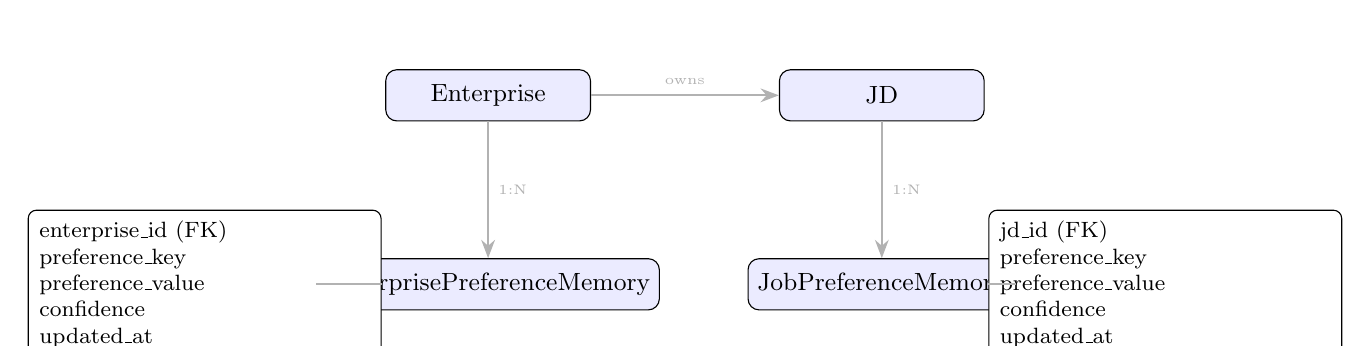
\begin{tikzpicture}[
  font=\small, >=Stealth,
  ent/.style={draw, rounded corners=4pt, fill=blue!8, align=center,
              minimum width=2.6cm, minimum height=0.65cm},
  attr/.style={draw, rounded corners=3pt, fill=white, align=left,
               text width=4.2cm, font=\footnotesize, inner sep=4pt},
  arr/.style={thick, color=gray!60},
]
\node[ent] (e) at (0,0)    {Enterprise};
\node[ent] (j) at (5.0,0)  {JD};
\node[ent] (ep) at (0,-2.4)   {EnterprisePreferenceMemory};
\node[ent] (jp) at (5.0,-2.4) {JobPreferenceMemory};

\node[attr] (ea) at (-3.6,-2.4) {enterprise\_id (FK)\\preference\_key\\preference\_value\\confidence\\updated\_at};
\node[attr] (ja) at (8.6,-2.4)  {jd\_id (FK)\\preference\_key\\preference\_value\\confidence\\updated\_at};

\draw[arr, ->] (e) -- node[right,font=\tiny]{1:N} (ep);
\draw[arr, ->] (j) -- node[right,font=\tiny]{1:N} (jp);
\draw[arr, -]  (ep) -- (ea);
\draw[arr, -]  (jp) -- (ja);
\draw[arr, ->] (e) -- node[above,font=\tiny]{owns} (j);
\end{tikzpicture}%
}
\caption{企业级 / 岗位级偏好的实体关系}
\label{fig:pref-er}
\end{figure}

\textbf{写入路径}由 LLM 主动调用 \texttt{save\_preference\_memory} 工具完成。工具描述特意做了行为约束：\textbf{只在用户明确表达硬性要求时调用，对试探性表达不调用}——把"什么是值得沉淀的偏好"的判断权交给 LLM 自己。\textbf{读取路径}则是在每次会话启动时从数据库重新加载偏好，拼成 markdown 列表写入 \texttt{state.preference\_context}，再 render 进 system prompt；放在 system prompt 而非 message 历史里，避免被摘要节点误压缩。

\subsection{Planning：ReAct 与 Plan-and-Execute 双范式}

ScoutAgent 同时实现了两种主流的 Agent 编排范式，分别承担不同的任务负载：\textbf{ReAct} 用于实时对话和单点提问，\textbf{Plan-and-Execute} 用于多步骤分析和报告生成。两者共享同一套工具与记忆，但执行结构截然不同。

\subsubsection{ReAct：经典 Reason–Act–Observe 循环}

Chat Graph 是经典的 ReAct 实现，LangGraph 用 \texttt{tools\_condition} 判断 LLM 输出里是否含 tool call 来决定走向。结构如图~\ref{fig:react-graph}~所示。每次进入 \texttt{chatbot} 节点都重新 \texttt{resolve\_tools(config)} 并 \texttt{bind\_tools}，实现"运行时绑定"；\texttt{dynamic\_tool\_node} 同样动态构造 \texttt{ToolNode(tools)}，与 chatbot 共用同一份工具列表。失败时通过 \texttt{ainvoke\_with\_fallback} 自动切换备用模型。

\begin{figure}[H]
\centering
\begin{tikzpicture}[
  font=\small, >=Stealth,
  state/.style={draw, rounded corners=4pt, fill=blue!10, align=center,
                minimum width=2.4cm, minimum height=0.7cm},
  cond/.style={draw, diamond, fill=yellow!18, aspect=2.6, align=center,
               minimum size=1.2cm, font=\footnotesize, inner sep=1pt},
  endN/.style={draw, rounded corners=4pt, fill=gray!12, align=center,
               minimum width=1.4cm, minimum height=0.7cm},
  arr/.style={->, thick, color=gray!60},
]
\node[state] (start) at (0,0) {START};
\node[state] (bot)   at (3.0,0) {chatbot\\\footnotesize bind tools};
\node[cond]  (cd)    at (6.4,0) {tools\_cond};
\node[state] (tn)    at (9.6,1.2)  {ToolNode};
\node[state] (sm)    at (9.6,-1.2) {maybe\_summarize};
\node[endN]  (en)    at (12.4,-1.2) {END};

\draw[arr] (start) -- (bot);
\draw[arr] (bot)   -- (cd);
\draw[arr] (cd) -- node[above,font=\tiny]{有工具} (tn);
\draw[arr] (cd) -- node[below,font=\tiny]{无工具} (sm);
\draw[arr] (tn.north) -- ++(0,0.5) -| (bot.north);
\draw[arr] (sm) -- (en);
\end{tikzpicture}
\caption{Chat Graph：ReAct 编排结构}
\label{fig:react-graph}
\end{figure}

\subsubsection{Plan-and-Execute：先规划、再逐步执行、再重规划}

Planning Graph 把任务拆成"先规划 $\to$ 逐步执行 $\to$ 再规划"三个阶段，每一步执行内部又是一个小型 ReAct 子图（图~\ref{fig:pae-graph}）。三个核心节点的角色见表~\ref{tab:pae-nodes}。

\begin{figure}[H]
\centering
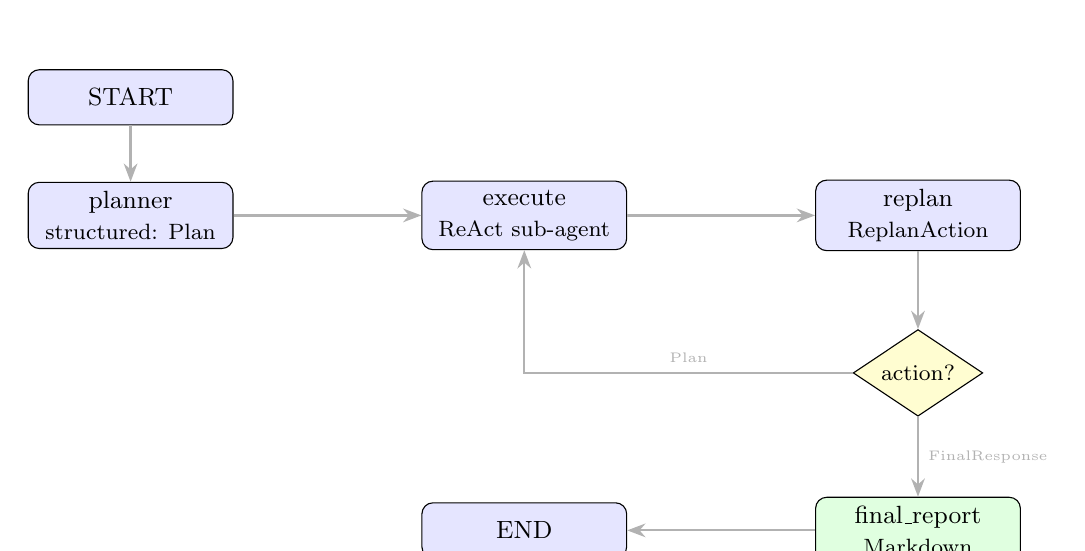
\begin{tikzpicture}[
  font=\small, >=Stealth,
  stepBox/.style={draw, rounded corners=4pt, fill=blue!10, align=center,
               minimum width=2.6cm, minimum height=0.7cm},
  dec/.style={draw, diamond, fill=yellow!18, aspect=2.4, align=center,
              minimum size=1.1cm, font=\footnotesize, inner sep=1pt},
  fin/.style={draw, rounded corners=4pt, fill=green!12, align=center,
              minimum width=2.6cm, minimum height=0.7cm},
  arr/.style={->, thick, color=gray!60},
]
\node[stepBox] (start) at (0,0) {START};
\node[stepBox] (pl)    at (0,-1.5) {planner\\\footnotesize structured: Plan};
\node[stepBox] (ex)    at (5.0,-1.5) {execute\\\footnotesize ReAct sub-agent};
\node[stepBox] (rp)    at (10.0,-1.5) {replan\\\footnotesize ReplanAction};
\node[dec]  (dc)    at (10.0,-3.5) {action?};
\node[fin]  (fr)    at (10.0,-5.5) {final\_report\\\footnotesize Markdown};
\node[stepBox] (en)    at (5.0,-5.5) {END};

\draw[arr] (start) -- (pl);
\draw[arr] (pl) -- (ex);
\draw[arr] (ex) -- (rp);
\draw[arr] (rp) -- (dc);
\draw[arr] (dc) -- node[above,font=\tiny]{Plan} (5.0,-3.5) -- (ex.south);
\draw[arr] (dc) -- node[right,font=\tiny]{FinalResponse} (fr);
\draw[arr] (fr) -- (en);
\end{tikzpicture}
\caption{Planning Graph：Plan-and-Execute 编排结构}
\label{fig:pae-graph}
\end{figure}

\begin{table}[H]
\centering
\renewcommand{\arraystretch}{1.3}
\caption{Plan-and-Execute 三个核心节点}
\label{tab:pae-nodes}
{\small
\begin{tabular}{L{2.4cm} L{3.4cm} L{3.6cm} L{3.0cm}}
\toprule
\textbf{节点} & \textbf{输入} & \textbf{输出（Pydantic）} & \textbf{作用} \\
\midrule
plan\_step & user input + 上下文 & Plan\{steps\} & 一次性产出有序计划 \\
execute\_step & 当前 plan 第一项 & past\_steps += [(step, result)] & 跑完一整步 ReAct 子循环 \\
replan\_step & 已执行 + 剩余计划 & ReplanAction (FinalResponse / Plan) & 决定继续还是收尾 \\
final\_report & 全部 past\_steps & 整合好的 Markdown & 输出最终结构化报告 \\
\bottomrule
\end{tabular}
}
\end{table}

关键设计上有四点值得强调：(1) \textbf{结构化输出}——\texttt{Plan / ReplanAction / FinalResponse} 都是 Pydantic 模型，用 \texttt{with\_structured\_output()} 强约束 LLM 输出；(2) \textbf{执行器是子图}——\texttt{execute\_step} 内部用 \texttt{create\_react\_agent} 临时构造 ReAct 子图跑当前步骤，并用 \texttt{MAX\_EXECUTOR\_ITERATIONS=15} 防止递归爆炸；(3) \textbf{append-only state}——\texttt{past\_steps} 用 \texttt{Annotated[list, operator.add]}，每个节点只追加自己的结果，避免并发写冲突；(4) \textbf{可中断恢复}——与 Chat Graph 共用同一个 Redis Checkpointer，长任务可跨进程恢复。

\subsubsection{两种范式的取舍}

ReAct 与 Plan-and-Execute 各有适用边界，我们从五个维度做对比（表~\ref{tab:react-vs-pae}）。最终在 ScoutAgent 中：\textbf{深度评估 Agent 默认走 ReAct}，可由用户在前端切换 Plan 模式后改用 Planning Graph。

\begin{table}[H]
\centering
\renewcommand{\arraystretch}{1.3}
\caption{ReAct 与 Plan-and-Execute 五维对比}
\label{tab:react-vs-pae}
\begin{tabular}{L{2.4cm} L{4.4cm} L{4.8cm}}
\toprule
\textbf{对比项} & \textbf{ReAct} & \textbf{Plan-and-Execute} \\
\midrule
规划粒度 & 隐式、每步重新决定 & 显式、提前一次性产出 \\
上下文消耗 & 每步把全部历史塞进去 & 计划字符串短，子执行器隔离 \\
适用任务 & 短交互、单跳工具调用 & 多步分析、跨工具协作、生成报告 \\
可解释性 & 隐藏在 message 流中 & plan 数组对外可见 \\
风险 & 长链路时易绕圈 & 计划过度刚性，需 replan 弥补 \\
\bottomrule
\end{tabular}
\end{table}

% ==================================================
% 第三章 关键算法与实验验证
% ==================================================
\section{关键算法与实验验证}\label{sec:exp}

\subsection{算法体系概览}

围绕"真实性验证 + 能力评估"的核心目标，本系统在算法侧落地了三项关键技术（图~\ref{fig:exp-overview}）：(1) 基于通义千问与思维链的\textbf{结构化信息抽取}，把非结构化简历与岗位描述转化为标准 JSON 画像；(2) 基于 Neo4j 的\textbf{技术知识图谱与 GraphRAG}，用图结构推理代替字符串匹配；(3) 基于 Qwen3.5 4B 的\textbf{简历过度包装检测}，采用 SFT 与 DPO 两阶段对齐输出可复核分析。每项技术都设计了与之配套的对照实验，下面分小节展开。

\begin{figure}[H]
\centering
\begin{tikzpicture}[
  font=\small, >=Stealth,
  src/.style={draw, rounded corners=4pt, fill=blue!8, align=center,
              minimum width=2.6cm, minimum height=0.7cm},
  algo/.style={draw, rounded corners=4pt, fill=green!10, align=center,
               minimum width=3.2cm, minimum height=0.85cm},
  result/.style={draw, rounded corners=4pt, fill=orange!12, align=center,
              minimum width=3.0cm, minimum height=0.7cm},
  arr/.style={->, thick, color=gray!60},
]
\node[src]    (s1) at (0,0)     {PDF 简历\\岗位文本};
\node[algo]   (a1) at (4.2,1.3) {\textbf{(1) CoT 抽取}\\Qwen + 思维链};
\node[algo]   (a2) at (4.2,0)   {\textbf{(2) GraphRAG}\\Neo4j 多跳推理};
\node[algo]   (a3) at (4.2,-1.3){\textbf{(3) SFT + DPO}\\Qwen3.5 4B};
\node[result] (o1) at (8.6,1.3) {结构化 JSON 画像};
\node[result] (o2) at (8.6,0)   {Good Fit / No Fit};
\node[result] (o3) at (8.6,-1.3){过度包装风险报告};

\draw[arr] (s1) -- (a1);
\draw[arr] (s1) -- (a2);
\draw[arr] (s1) -- (a3);
\draw[arr] (a1) -- (o1);
\draw[arr] (a2) -- (o2);
\draw[arr] (a3) -- (o3);
\draw[arr, dashed] (a1) -- node[right,font=\tiny]{为下游提供画像} (a2);
\end{tikzpicture}
\caption{三项关键算法及其输入输出关系}
\label{fig:exp-overview}
\end{figure}

\subsection{结构化信息抽取（Qwen API + CoT）}

\subsubsection{方法要点}

岗位描述与简历多为非结构化文本，直接匹配噪声大。我们首先用 \texttt{pdfplumber} 把简历 PDF 转为纯文本，再调用\textbf{通义千问（Qwen）API}，配合\textbf{思维链（Chain of Thought）}采用"由粗到细"的两阶段抽取：第一阶段先做\textbf{语义分块}（简历六类区块；JD 拆为教育/技能/经历要求等），第二阶段在每个块上按 \textbf{Schema} 输出 JSON。简历侧从 NER 14 类标签中选取核心映射：\texttt{DESIGNATION} $\to$ 期望职位、\texttt{EDUCATION} $\to$ 教育、\texttt{SKILL} $\to$ 专业技能、\texttt{EXPERIENCE} + \texttt{COMPANY} $\to$ 实习/工作经历，最终输出统一的候选人画像 JSON。

\subsubsection{评测设置与结果}

简历评测使用 Kaggle 公开 Resume NER Training Dataset 中的 \textbf{5,960} 个样本；岗位评测使用约 \textbf{100} 条真实招聘平台非结构化文本与人工提取特征。由于系统输出为 JSON 聚合字段，与序列标注位对齐困难，验证逻辑采用"语义关联比对"——抽取内容与原文标注位置文本相似且信息一致即计为有效召回，各核心维度加权平均，最终汇报 Precision、Recall、F1 三项指标（表~\ref{tab:exp-extraction}）。

\begin{table}[H]
\centering
\renewcommand{\arraystretch}{1.35}
\caption{结构化信息抽取性能对比（简历评测，n = 5{,}960）}
\label{tab:exp-extraction}
\begin{tabular}{L{6.0cm} C{2.4cm} C{2.4cm} C{2.4cm}}
\toprule
\textbf{方案} & \textbf{Precision (\%)} & \textbf{Recall (\%)} & \textbf{F1 (\%)} \\
\midrule
Naive LLM 直接抽取（Zero-shot） & 68 & 64 & 66 \\
\textbf{Qwen API + CoT 任务分解（本系统）} & \textbf{79} & \textbf{76} & \textbf{78} \\
\bottomrule
\end{tabular}
\end{table}

\textbf{结论}：相对 Zero-shot 直接抽取，CoT 任务分解将 F1 从 66\% 提升到 78\%，验证了"分块定位 + 局部 Schema 抽取"对长文本"中间信息丢失"问题的缓解效果。

\subsection{技术知识图谱与 GraphRAG 匹配增强}

\subsubsection{图谱构建}

技术知识图谱存储于 \textbf{Neo4j}，节点以技术 Tag 为主，关系类型与权重经反复调试后固定为表~\ref{tab:kg-rel} 三类。其中跳数衰减满足 $\delta(1)=1.0,\delta(2)=0.5,\delta(3)=0.25$，三跳即截断。

\begin{table}[H]
\centering
\renewcommand{\arraystretch}{1.35}
\caption{知识图谱关系类型与权重}
\label{tab:kg-rel}
\begin{tabular}{L{3.0cm} L{2.8cm} C{1.4cm} L{4.6cm}}
\toprule
\textbf{关系名称} & \textbf{关系类别} & \textbf{$w(r)$} & \textbf{业务语义} \\
\midrule
\texttt{BELONGS\_TO} & 技术归属 / 分类 & 5.0 & 大类—细分，用于多跳扩展 \\
\texttt{DEPENDS\_ON} & 技术依赖 & 3.0 & 强约束依赖链，一跳优先 \\
\texttt{RELATED\_TO} & 共现关联 & 1.0 & 弱关联，权重最低 \\
\bottomrule
\end{tabular}
\end{table}

数据来源覆盖四个渠道：\textbf{Stack Overflow Tag Synonyms} 提供异名归一、\textbf{GitHub Awesome 系列}（Awesome-Python / Go / Java 等）提供 BELONGS\_TO 层次、\textbf{Maven 与 PyPI 制品元数据}提供 DEPENDS\_ON、\textbf{热门仓库 Topics 共现统计}提供 RELATED\_TO（带阈值抑制噪声）；额外通过 GitHub API 爬取 Top 约 5{,}000 仓库标签用于共现与覆盖分析。最终全图规模约为\textbf{核心实体 4,800 个、三元组 32,000 条}。

\subsubsection{GraphRAG 匹配判别流程}

完整的"解析 $\to$ 图谱 $\to$ 判别"流程如图~\ref{fig:graphrag}~所示。完整 JD/CV 文本先经 \textbf{DeepSeek Chat} 解析为 JSON，再抽取技能列表去重；随后做别名归一并通过 Neo4j \textbf{最短路径 $\le$3 跳} 生成"KG 技能覆盖分析"文本；最后把 JSON 与 KG 文本一并送入 LLM 输出 Good Fit / No Fit。右侧对照分支为"纯 LLM 仅 JSON"，与本路径仅在是否注入 KG 文本上不同，保证对照公平。

\begin{figure}[H]
\centering
\begin{tikzpicture}[
  font=\small, >=Stealth,
  stepBox/.style={draw, rounded corners=4pt, fill=blue!8, align=center,
               minimum width=3.6cm, minimum height=0.7cm},
  kg/.style={draw, rounded corners=4pt, fill=green!10, align=center,
             minimum width=3.6cm, minimum height=0.7cm},
  ctrl/.style={draw, rounded corners=4pt, fill=orange!12, align=center,
               minimum width=3.6cm, minimum height=0.7cm},
  result/.style={draw, rounded corners=4pt, fill=red!10, align=center,
              minimum width=3.0cm, minimum height=0.7cm},
  arr/.style={->, thick, color=gray!60},
]
\node[stepBox]   (a) at (0,0)    {JD/CV 原文};
\node[stepBox]   (b) at (0,-1.5) {LLM 解析\\\footnotesize parse\_jd / parse\_cv};
\node[stepBox]   (c) at (0,-3.0) {结构化 JSON};
\node[stepBox]   (d) at (0,-4.5) {抽取技能列表去重};
\node[kg]     (e) at (0,-6.0) {别名归一 + Neo4j 最短路径 $\le$3 跳};
\node[kg]     (f) at (0,-7.5) {KG 技能覆盖分析文本};
\node[result] (g) at (0,-9.0) {LLM + KG\\\footnotesize Good Fit / No Fit};

\node[ctrl]   (h) at (6.4,-6.0) {对照分支：纯 LLM};
\node[result] (i) at (6.4,-9.0) {LLM only\\\footnotesize Good Fit / No Fit};

\draw[arr] (a)--(b); \draw[arr] (b)--(c);
\draw[arr] (c)--(d); \draw[arr] (d)--(e);
\draw[arr] (e)--(f); \draw[arr] (f)--(g);
\draw[arr, dashed] (c.east) -- ++(2.5,0) |- (h.west);
\draw[arr, dashed] (h)--(i);
\end{tikzpicture}
\caption{GraphRAG 匹配判别流程及对照分支}
\label{fig:graphrag}
\end{figure}

\subsubsection{实验一：留一技能补全}

第一组实验在 \texttt{jd\_keywords} 上做 \textbf{Leave-One-Out}（LOO）：每次抽掉一个目标技能，用其余技能作为上下文，检验目标技能是否进入推荐 Top-K。基线包括同源 Neo4j 统计的\textbf{共现矩阵}与\textbf{全局词频}两种朴素方法，指标为 Hit@5 / Hit@10 / MRR（表~\ref{tab:exp-loo}）。

\begin{table}[H]
\centering
\renewcommand{\arraystretch}{1.35}
\caption{留一技能补全的对照结果}
\label{tab:exp-loo}
\begin{tabular}{L{6.4cm} C{2.0cm} C{2.0cm} C{2.0cm}}
\toprule
\textbf{方法} & \textbf{Hit@5 (\%)} & \textbf{Hit@10 (\%)} & \textbf{MRR (\%)} \\
\midrule
\textbf{知识图谱多跳推荐（本系统）} & \textbf{23.32} & 34.69 & \textbf{15.99} \\
共现矩阵基线（cooccurrence） & 22.46 & \textbf{35.59} & 14.07 \\
全局词频基线（freq） & 19.61 & 32.06 & 11.99 \\
\bottomrule
\end{tabular}
\end{table}

\textbf{结论}：图谱多跳推荐在 Hit@5 与 MRR 上均优于共现与词频基线，证明了图结构在"语义近邻"识别上的优势；Hit@10 上略低于共现矩阵，原因是共现统计在长尾时召回更广，但这部分召回的相关性更弱（MRR 较低也佐证这一点）。

\subsubsection{实验二：JD/CV 匹配二分类}

第二组实验直接在匹配判别任务上评测。数据来自 Hugging Face 公开数据集 \texttt{facehuggerapoorv/resume-jd-match}（约 8k 行），清洗后约六千余条有效记录，字段包含 \texttt{cv}、\texttt{jd}、\texttt{label}（No Fit / Good Fit / Potential Fit）、\texttt{cv\_keywords}、\texttt{jd\_keywords}。评测时\textbf{排除 Potential Fit}，仅在 Good Fit 与 No Fit 上做二分类，对比纯 LLM 与 LLM+KG（表~\ref{tab:exp-match}）。

\begin{table}[H]
\centering
\renewcommand{\arraystretch}{1.35}
\caption{JD/CV 匹配二分类准确率（剔除 Potential Fit）}
\label{tab:exp-match}
\begin{tabular}{L{8.0cm} C{3.0cm}}
\toprule
\textbf{方法} & \textbf{准确率 (\%)} \\
\midrule
纯 LLM（结构化 JSON $\to$ 预测） & 74.3 \\
\textbf{LLM + KG（JSON + KG 覆盖文本 $\to$ 预测）} & \textbf{85.2} \\
\bottomrule
\end{tabular}
\end{table}

\textbf{结论}：相对纯 LLM 基线，引入 KG 覆盖分析后准确率提升约 \textbf{10.9 个百分点}，证明 GraphRAG 在"语义 + 结构"双重对齐上的有效性。

\subsection{简历过度包装检测（SFT + DPO）}

\subsubsection{任务定义}

本任务关注简历中的\textbf{语义夸大}（层级与事实不符），而非"AI 生成检测"或文风分类；输出需要可复核——不仅给出结论，还要列出疑点与建议的面试追问，让 HR 可以回落到原文核对。

\subsubsection{数据合成}

数据与图谱评测同源，清洗对齐后通过 \texttt{make\_rl\_dataset.py} 管道生成 JSONL（\texttt{prompt} / \texttt{chosen} / \texttt{rejected}）；仅保留 Good Fit 与 Potential Fit，排除 No Fit，避免对原本就不匹配的简历"强行拔高"。划分采用固定随机种子，\textbf{训练集 1{,}000 条、测试集 200 条}（约 83\% / 17\%）。三种合成策略与 DPO 字段的语义见表~\ref{tab:dpo-strategy}。

\begin{table}[H]
\centering
\renewcommand{\arraystretch}{1.3}
\caption{DPO 数据合成策略与字段语义}
\label{tab:dpo-strategy}
{\small
\begin{tabular}{L{2.6cm} L{2.6cm} L{6.4cm}}
\toprule
\textbf{策略} & \textbf{适用标签} & \textbf{摘要} \\
\midrule
inflate\_weak & Potential Fit & 高级词汇堆砌、职责夸大，故意留资历或技术矛盾 \\
inflate\_strong & 部分 Good Fit & 指标夸大 5--20 倍、独揽团队成果等 \\
authentic & 部分 Good Fit & 真实 CV；chosen 客观、rejected 模拟无理挑刺 \\
\midrule
\textbf{字段} & \multicolumn{2}{l}{\textbf{含义}} \\
\midrule
prompt & \multicolumn{2}{l}{含 JD 与（策略处理后的）CV 的研判指令} \\
chosen & \multicolumn{2}{l}{应提高概率：正确识别夸大或公正评价真实简历} \\
rejected & \multicolumn{2}{l}{应压低概率：误判或挑刺} \\
\bottomrule
\end{tabular}
}
\end{table}

\subsubsection{训练顺序与评测协议}

基座模型选用 \textbf{Qwen3.5 4B}，兼顾算力与推理效率。训练顺序为 \textbf{SFT $\to$ DPO}：SFT 让模型先学会固定的分析范式与输出结构，DPO 在此基础上做成对偏好对齐，抬高可信分析、压低误判。评测时主指标为 \textbf{Pairwise Accuracy}，并辅以传统的 Accuracy 与宏平均 F1（与 \texttt{is\_fabricated} 元数据对齐），基线为同规模的 \textbf{Qwen API Zero-shot}。

\begin{table}[H]
\centering
\renewcommand{\arraystretch}{1.35}
\caption{过度包装检测结果（测试集 n = 200）}
\label{tab:exp-fabrication}
\begin{tabular}{L{6.0cm} C{2.2cm} C{2.2cm} C{2.6cm}}
\toprule
\textbf{方法} & \textbf{Accuracy (\%)} & \textbf{F1 (\%)} & \textbf{Pairwise Acc (\%)} \\
\midrule
直接调用 Qwen API（Zero-shot） & 70.5 & 67.8 & 73.5 \\
\textbf{本项目：SFT + DPO} & \textbf{83.0} & \textbf{80.5} & \textbf{88.5} \\
\bottomrule
\end{tabular}
\end{table}

\textbf{结论}：在三项指标上均显著优于 Zero-shot 基线，其中 Pairwise Accuracy 提升 \textbf{15 个百分点}，验证了"SFT 定型 + DPO 对齐"两阶段策略对小模型的适用性。

\subsection{微调模型服务化部署}

考虑到主站云主机内存受限，过度包装检测模型不适合与业务后端共置。我们将 SFT+DPO 后的 Qwen3.5 4B 权重部署到 \textbf{AutoDL} GPU 实例（NVIDIA RTX 5090，Ubuntu 22.04），以独立 \textbf{FastAPI} 进程加载并对外暴露 HTTP 接口；阿里云 ECS 与 AutoDL 之间通过 \textbf{SSH 端口转发}打通，主业务后端访问 \texttt{127.0.0.1:9000/predict} 即可调用远端推理服务。具体的拓扑细节将在第~\ref{sec:tech}~章统一展开。

% ==================================================
% 第四章 技术栈与部署
% ==================================================
\section{技术栈与部署}\label{sec:tech}

\subsection{总体架构}

ScoutAgent 整体由\textbf{前端 SPA、后端 API/Agent 服务、三类数据存储}组成，统一通过 Docker Compose 编排部署。整体拓扑如图~\ref{fig:tech-overview}~所示。

\begin{figure}[H]
\centering
\begin{tikzpicture}[
  font=\small, >=Stealth,
  layer/.style={draw, rounded corners=4pt, align=center,
                minimum width=12.0cm, minimum height=0.85cm},
  fe/.style={layer, fill=blue!8},
  be/.style={layer, fill=orange!12},
  ag/.style={layer, fill=green!10},
  st/.style={draw, rounded corners=4pt, fill=purple!10, align=center,
             minimum width=3.6cm, minimum height=0.85cm},
  arr/.style={->, thick, color=gray!60},
]
\node[fe] (fe) at (0,0) {Frontend (Browser SPA)\\\footnotesize React 18 · TypeScript · Vite 5 · React Router 7 · Nginx};
\node[be] (be) at (0,-1.4) {Backend API (FastAPI · Uvicorn)\\\footnotesize 路由层 · 鉴权 · 业务服务 · 流式输出};
\node[ag] (ag) at (0,-2.8) {Agent Runtime\\\footnotesize LangGraph · LangChain · OpenAI 兼容 LLM · MCP / Skills};

\node[st] (pg) at (-4.0,-4.5) {PostgreSQL 16\\\footnotesize 业务结构化数据};
\node[st] (rd) at (0,-4.5)    {Redis Stack\\\footnotesize 会话 / 检查点 / 缓存};
\node[st] (nj) at (4.0,-4.5)  {Neo4j 5\\\footnotesize 技术知识图谱};

\draw[arr] (fe) -- node[right,font=\tiny]{REST + SSE (JWT Bearer)} (be);
\draw[arr] (be) -- (ag);
\draw[arr] (ag) -- (pg);
\draw[arr] (ag) -- (rd);
\draw[arr] (ag) -- (nj);
\end{tikzpicture}
\caption{ScoutAgent 总体技术架构}
\label{fig:tech-overview}
\end{figure}

\subsection{前端}

前端是一个标准的 React 18 + TypeScript SPA，所有业务路由都受 \texttt{ProtectedRoute} 保护，401 自动登出回到登录页。长任务（评估、对话）通过 SSE 流式接收，Markdown 内容统一用 \texttt{react-markdown} + \texttt{remark-gfm} 渲染。生产环境构建产物由 \texttt{nginx:alpine} 静态托管并反向代理到后端（表~\ref{tab:tech-fe}）。

\begin{table}[H]
\centering
\renewcommand{\arraystretch}{1.3}
\caption{前端技术栈}
\label{tab:tech-fe}
\begin{tabular}{L{3.0cm} L{8.6cm}}
\toprule
\textbf{维度} & \textbf{技术选型} \\
\midrule
UI 框架 & React 18 \\
语言 & TypeScript 5 \\
构建工具 & Vite 5（\texttt{@vitejs/plugin-react}） \\
路由 & React Router DOM 7 \\
内容渲染 & \texttt{react-markdown} + \texttt{remark-gfm}（评估报告 / 对话内容）\\
通信 & \texttt{fetch} + REST，长任务用 SSE 流式接收 \\
静态托管 & 生产由 \texttt{nginx:alpine} 提供静态资源与反向代理 \\
\bottomrule
\end{tabular}
\end{table}

\subsection{后端 API}

后端基于 FastAPI + Uvicorn 多 worker 部署，数据访问采用 SQLAlchemy ORM + \texttt{psycopg[binary]} 驱动，库表迁移由 Alembic 管理。鉴权使用 JWT（PyJWT）+ Bearer Token，简历 PDF 由 PyMuPDF 解析（多模块同名 \texttt{pdfplumber} 仅在抽取实验中使用），流式响应通过 \texttt{stream\_buffer.py} 维护，全链路 Tracing 接入 LangSmith（表~\ref{tab:tech-be}）。

\begin{table}[H]
\centering
\renewcommand{\arraystretch}{1.3}
\caption{后端 API 技术栈}
\label{tab:tech-be}
\begin{tabular}{L{3.0cm} L{8.6cm}}
\toprule
\textbf{维度} & \textbf{技术选型} \\
\midrule
运行时 & Python（\texttt{python:slim} 容器） \\
Web 框架 & FastAPI \\
ASGI 服务器 & Uvicorn（\texttt{--workers 2}） \\
数据访问 & SQLAlchemy ORM + \texttt{psycopg[binary]} \\
迁移 & Alembic \\
配置管理 & Pydantic / \texttt{pydantic-settings} + \texttt{python-dotenv} \\
鉴权 & JWT（PyJWT）+ Bearer Token \\
文件解析 & PyMuPDF；上传走 \texttt{python-multipart} \\
流式响应 & SSE（\texttt{stream\_buffer.py}） \\
可观测性 & LangSmith Tracing \\
\bottomrule
\end{tabular}
\end{table}

\subsection{Agent 框架}

Agent 框架是后端的核心，所有智能体能力都通过 LangGraph 编排（表~\ref{tab:tech-ag}）。LLM 接入统一走 OpenAI 兼容接口（\texttt{langchain-openai} + \texttt{openai} SDK），默认模型为 Kimi K2.5；token 计算用 \texttt{tiktoken}；记忆侧的状态/检查点由 LangGraph Checkpoint Redis 持久化；工具扩展同时支持 MCP 协议与自研 Skills 模块；知识图谱检索使用 Neo4j 官方 Python Driver 直连。

\begin{table}[H]
\centering
\renewcommand{\arraystretch}{1.3}
\caption{Agent 框架技术栈}
\label{tab:tech-ag}
\begin{tabular}{L{3.0cm} L{8.6cm}}
\toprule
\textbf{维度} & \textbf{技术选型} \\
\midrule
编排框架 & LangGraph（多阶段 Workflow、Planning、状态机） \\
基础能力 & LangChain（Prompt / Tool / Chain 抽象） \\
LLM 接入 & OpenAI 兼容接口（\texttt{langchain-openai} + \texttt{openai}） \\
Token 计算 & \texttt{tiktoken} \\
状态 / 记忆 & LangGraph Checkpoint，由 Redis 持久化 \\
工具扩展 & MCP（\texttt{langchain-mcp-adapters} + \texttt{mcp}）+ 自研 Skills \\
知识图谱检索 & Neo4j 官方 Python Driver \\
业务模块 & \texttt{agent/planning, assessment, chat, resume, skills, tools} \\
\bottomrule
\end{tabular}
\end{table}

\subsection{数据存储}

三类存储承担不同职责：PostgreSQL 持久化业务结构化数据、Redis 承担会话与检查点、Neo4j 提供 GraphRAG 检索（表~\ref{tab:tech-store}）。

\begin{table}[H]
\centering
\renewcommand{\arraystretch}{1.3}
\caption{数据存储}
\label{tab:tech-store}
\begin{tabular}{L{2.4cm} L{4.4cm} L{5.0cm}}
\toprule
\textbf{存储} & \textbf{版本 / 镜像} & \textbf{用途} \\
\midrule
PostgreSQL & \texttt{postgres:16} / \texttt{postgres:alpine} & 企业、JD、候选人、CV、申请、评估等结构化业务数据 \\
Redis & \tk{redis/redis-stack-server:latest} & 会话状态、缓存、LangGraph Checkpoint 持久化 \\
Neo4j & \texttt{neo4j:5} / \texttt{neo4j:latest} & 技术知识图谱（技能、框架、上下位关系），支撑 GraphRAG \\
\bottomrule
\end{tabular}
\end{table}

\subsection{部署}

系统采用 Docker Compose 双 compose 编排——开发用 \texttt{docker-compose.yml}、生产用 \texttt{docker-compose.prod.yml}（表~\ref{tab:tech-deploy}）。各服务均配置 \texttt{healthcheck}（\texttt{pg\_isready}、\texttt{redis-cli ping}、Neo4j HTTP、\texttt{/api/health}），生产 compose 进一步对 PostgreSQL 与 Neo4j 做 JVM/缓冲调优并设置 memory limits。

\begin{table}[H]
\centering
\renewcommand{\arraystretch}{1.3}
\caption{部署方案}
\label{tab:tech-deploy}
\begin{tabular}{L{2.6cm} L{9.2cm}}
\toprule
\textbf{维度} & \textbf{方案} \\
\midrule
容器编排 & Docker Compose（开发 / 生产双文件） \\
服务拓扑 & frontend (Nginx 80) $\to$ backend (FastAPI 8000) $\to$ postgres / neo4j / redis \\
镜像构建 & 后端基于 \texttt{python:slim}；前端 \texttt{node:18-alpine} 多阶段构建后由 \texttt{nginx:alpine} 托管 \\
健康检查 & 各服务均配置 healthcheck \\
资源限制 & 生产 compose 设置 memory limits/reservations，并对 PG/Neo4j 做调优 \\
配置注入 & \texttt{.env} + 环境变量（数据库连接、JWT、LLM Key、Neo4j 凭据等） \\
本地一键启动 & \texttt{run.sh} 串行启动 Neo4j $\to$ PG/Redis $\to$ Backend $\to$ Frontend \\
\bottomrule
\end{tabular}
\end{table}

\subsection{云端运行环境与 AutoDL 推理隧道}

主站部署在阿里云 ECS（Ubuntu 22.04 LTS、2 核 / 4 GB），Nginx、SSL 证书与反向代理通过宝塔面板管理；公网入口通过弹性公网 IP 对外提供。\textbf{过度包装检测模型}的推理服务部署在 AutoDL GPU（NVIDIA RTX 5090）上，通过\textbf{SSH 本地端口转发}将 AutoDL 上 \texttt{127.0.0.1:8000} 的 FastAPI 映射到 ECS 本机 \texttt{127.0.0.1:9000}（图~\ref{fig:deploy-topo}）。这种"主业务 + AutoDL 自托管推理"的混合架构有两个好处：(1) 避免在 2 GB 内存的 ECS 上加载 4B 级权重导致 OOM；(2) 推理算力按任务时段租用，不为整站长期绑定高价 GPU。

\begin{figure}[H]
\centering
\resizebox{0.98\textwidth}{!}{%
\begin{tikzpicture}[
  font=\small, >=Stealth,
  inet/.style={draw, rounded corners=4pt, fill=blue!8, align=center, minimum width=2.5cm, minimum height=0.75cm},
  box/.style ={draw, rounded corners=3pt, fill=white, align=center, minimum width=2.85cm, minimum height=0.72cm},
  arr/.style={->, thick, color=gray!60},
]
\node[inet] (net) at (0,0) {Internet};
\node[font=\footnotesize\itshape, anchor=east, align=right] at (-3.2,-0.95)
  {Ubuntu 22.04 LTS · 2 核 / 4 GB};

\node[box, fill=yellow!12] (bt) at (-6.2,-3.4) {宝塔面板\\运维入口};
\node[box, fill=orange!10] (nx) at (0,-3.4) {Nginx\\:80 / :443};

\node[box, fill=blue!8] (fe) at (-6.2,-6.2) {静态资源\\Vite build};
\node[box, fill=blue!8, minimum width=3.0cm] (be) at (-0.85,-6.2) {主业务后端\\Uvicorn :8000};
\node[draw, rounded corners=3pt, fill=gray!12, align=center, font=\footnotesize,
      minimum width=2.5cm, minimum height=0.95cm, inner sep=3pt] (loc) at (4.15,-6.2)
  {\texttt{127.0.0.1:9000}\\[-2pt]\tiny 本机环回};
\node[draw, dashed, rounded corners=6pt, fill=red!7, align=center, inner sep=5pt,
      minimum width=3.6cm, minimum height=1.5cm] (adl) at (9.85,-6.2)
  {\textbf{AutoDL}\\[1pt]FastAPI \texttt{:8000} · \texttt{/predict}\\[1pt]\footnotesize Qwen3.5 4B · RTX 5090};

\node[box, fill=green!8, minimum width=2.55cm] (pg) at (-3.4,-9.2) {PostgreSQL\\:5432};
\node[box, fill=green!8, minimum width=2.55cm] (nj) at (3.4,-9.2)  {Neo4j\\:7687};

\draw[arr] (net.south) -- (0,-0.55);
\draw[arr] (0,-0.55) -- (0,-1.85) -- (nx.north);

\draw[arr, dashed, color=gray!45] (bt.east) -- node[above,font=\tiny,yshift=2pt]{运维配置} (nx.west);

\coordinate (nxsplit) at (0,-5.05);
\draw[arr] (nx.south) -- (nxsplit);
\draw[arr] (nxsplit) -| node[pos=0.42, below, font=\tiny, yshift=-1pt]{站点根} (fe.north);
\draw[arr] (nxsplit) -- node[right, font=\tiny, xshift=4pt]{反代} (be.north);

\coordinate (dbfork) at (-0.85,-7.35);
\draw[arr] (be.south) -- (dbfork);
\draw[arr] (dbfork) -| (pg.north);
\draw[arr] (dbfork) -| (nj.north);

\draw[arr] (be.east) -- node[above, font=\tiny, yshift=2pt]{HTTP} (loc.west);
\draw[arr, dashed, color=purple!55, thick] (loc.east) --
  node[above, font=\scriptsize, yshift=3pt]{SSH 转发} (adl.west);
\end{tikzpicture}%
}
\caption{部署拓扑：Web、数据层与 AutoDL 推理（SSH 端口转发）}
\label{fig:deploy-topo}
\end{figure}

SSH 隧道的典型命令为 \texttt{ssh -L 9000:127.0.0.1:8000 root@<AutoDL 实例地址>}；生产环境可使用 \texttt{autossh} 或在 \texttt{systemd} 中注册服务以保持自动重连。其余智能体（如 JD-CV 匹配、深度对话）继续通过 OpenAI 兼容接口调用云端 Kimi 模型，与上述自托管 Qwen 推理路径在 \texttt{.env} 中分别配置 Base URL 即可并行存在。

% ==================================================
% 第五章 系统功能展示
% ==================================================
\section{系统功能展示}\label{sec:func}

\subsection{页面总览}

ScoutAgent 前端基于 React 18 + TypeScript + Vite + React Router 7 构建，由左侧固定的图标导航栏串联起 5 个核心页面，所有页面共享 JWT 鉴权、SSE 流式通信与统一的 Markdown 渲染体系（表~\ref{tab:page-overview}）。

\begin{table}[H]
\centering
\renewcommand{\arraystretch}{1.3}
\caption{ScoutAgent 五大业务页面}
\label{tab:page-overview}
\begin{tabular}{C{0.6cm} L{3.4cm} L{3.4cm} L{4.6cm}}
\toprule
\textbf{\#} & \textbf{页面} & \textbf{路由} & \textbf{一句话定位} \\
\midrule
1 & 企业与岗位管理 & \texttt{/enterprises} & 招聘信息的"源头"：维护客户、JD 与投递关系 \\
2 & 候选人管理 & \texttt{/candidates} & 简历的"档案库"：PDF $\to$ 结构化 Profile \\
3 & 批量化评估 & \texttt{/assess} & 全局视角的"流水线评估"：批量打分与筛选 \\
4 & \textbf{深度评估 Agent} & \tk{/assess/assistant} & \textbf{对话式深评：多轮、可追溯、有记忆} \\
5 & Eval 系统 & \texttt{/eval} & 离线评测中心：跑评测、看指标、做回归 \\
\bottomrule
\end{tabular}
\end{table}

五个页面在业务上构成闭环：第 1、2 页提供"原料"（企业/JD 与候选人简历），第 3 页做"粗筛"，第 4 页做"精评 + 经验沉淀"，第 5 页保证"模型升级不退化"（图~\ref{fig:page-loop}）。

\begin{figure}[H]
\centering
\resizebox{\textwidth}{!}{%
\begin{tikzpicture}[
  font=\small, >=Stealth,
  pg/.style={draw, rounded corners=4pt, fill=blue!8, align=center,
             minimum width=2.6cm, minimum height=0.85cm},
  hub/.style={draw, rounded corners=4pt, fill=green!12, align=center,
              minimum width=3.2cm, minimum height=0.85cm},
  arr/.style={->, thick, color=gray!60},
]
\node[pg]  (cand) at (-5.6,1.2) {候选人管理\\\footnotesize PDF $\to$ JSON};
\node[pg]  (ent)  at (-5.6,-1.2) {企业与岗位\\\footnotesize JD / 投递};
\node[pg]  (asm)  at (-1.0,0)    {批量化评估\\\footnotesize 流水线打分};
\node[hub] (assi) at (3.6,0)     {深度评估 Agent\\\footnotesize ReAct + Planning};
\node[pg]  (pref) at (3.6,-2.2)  {偏好沉淀\\\footnotesize 企业/岗位级};
\node[pg]  (eval) at (8.0,0)     {Eval 系统\\\footnotesize 回归 + 同步};

\draw[arr] (cand) -- (asm);
\draw[arr] (ent)  -- (asm);
\draw[arr] (asm)  -- (assi);
\draw[arr] (assi) -- (eval);
\draw[arr] (assi.south) -- (pref.north);
\draw[arr, dashed] (pref.west) -- ++(-3.5,0) |- (ent.east);
\end{tikzpicture}%
}
\caption{五大页面的业务闭环}
\label{fig:page-loop}
\end{figure}

\subsection{企业与岗位管理}

\begin{figure}[H]
\centering
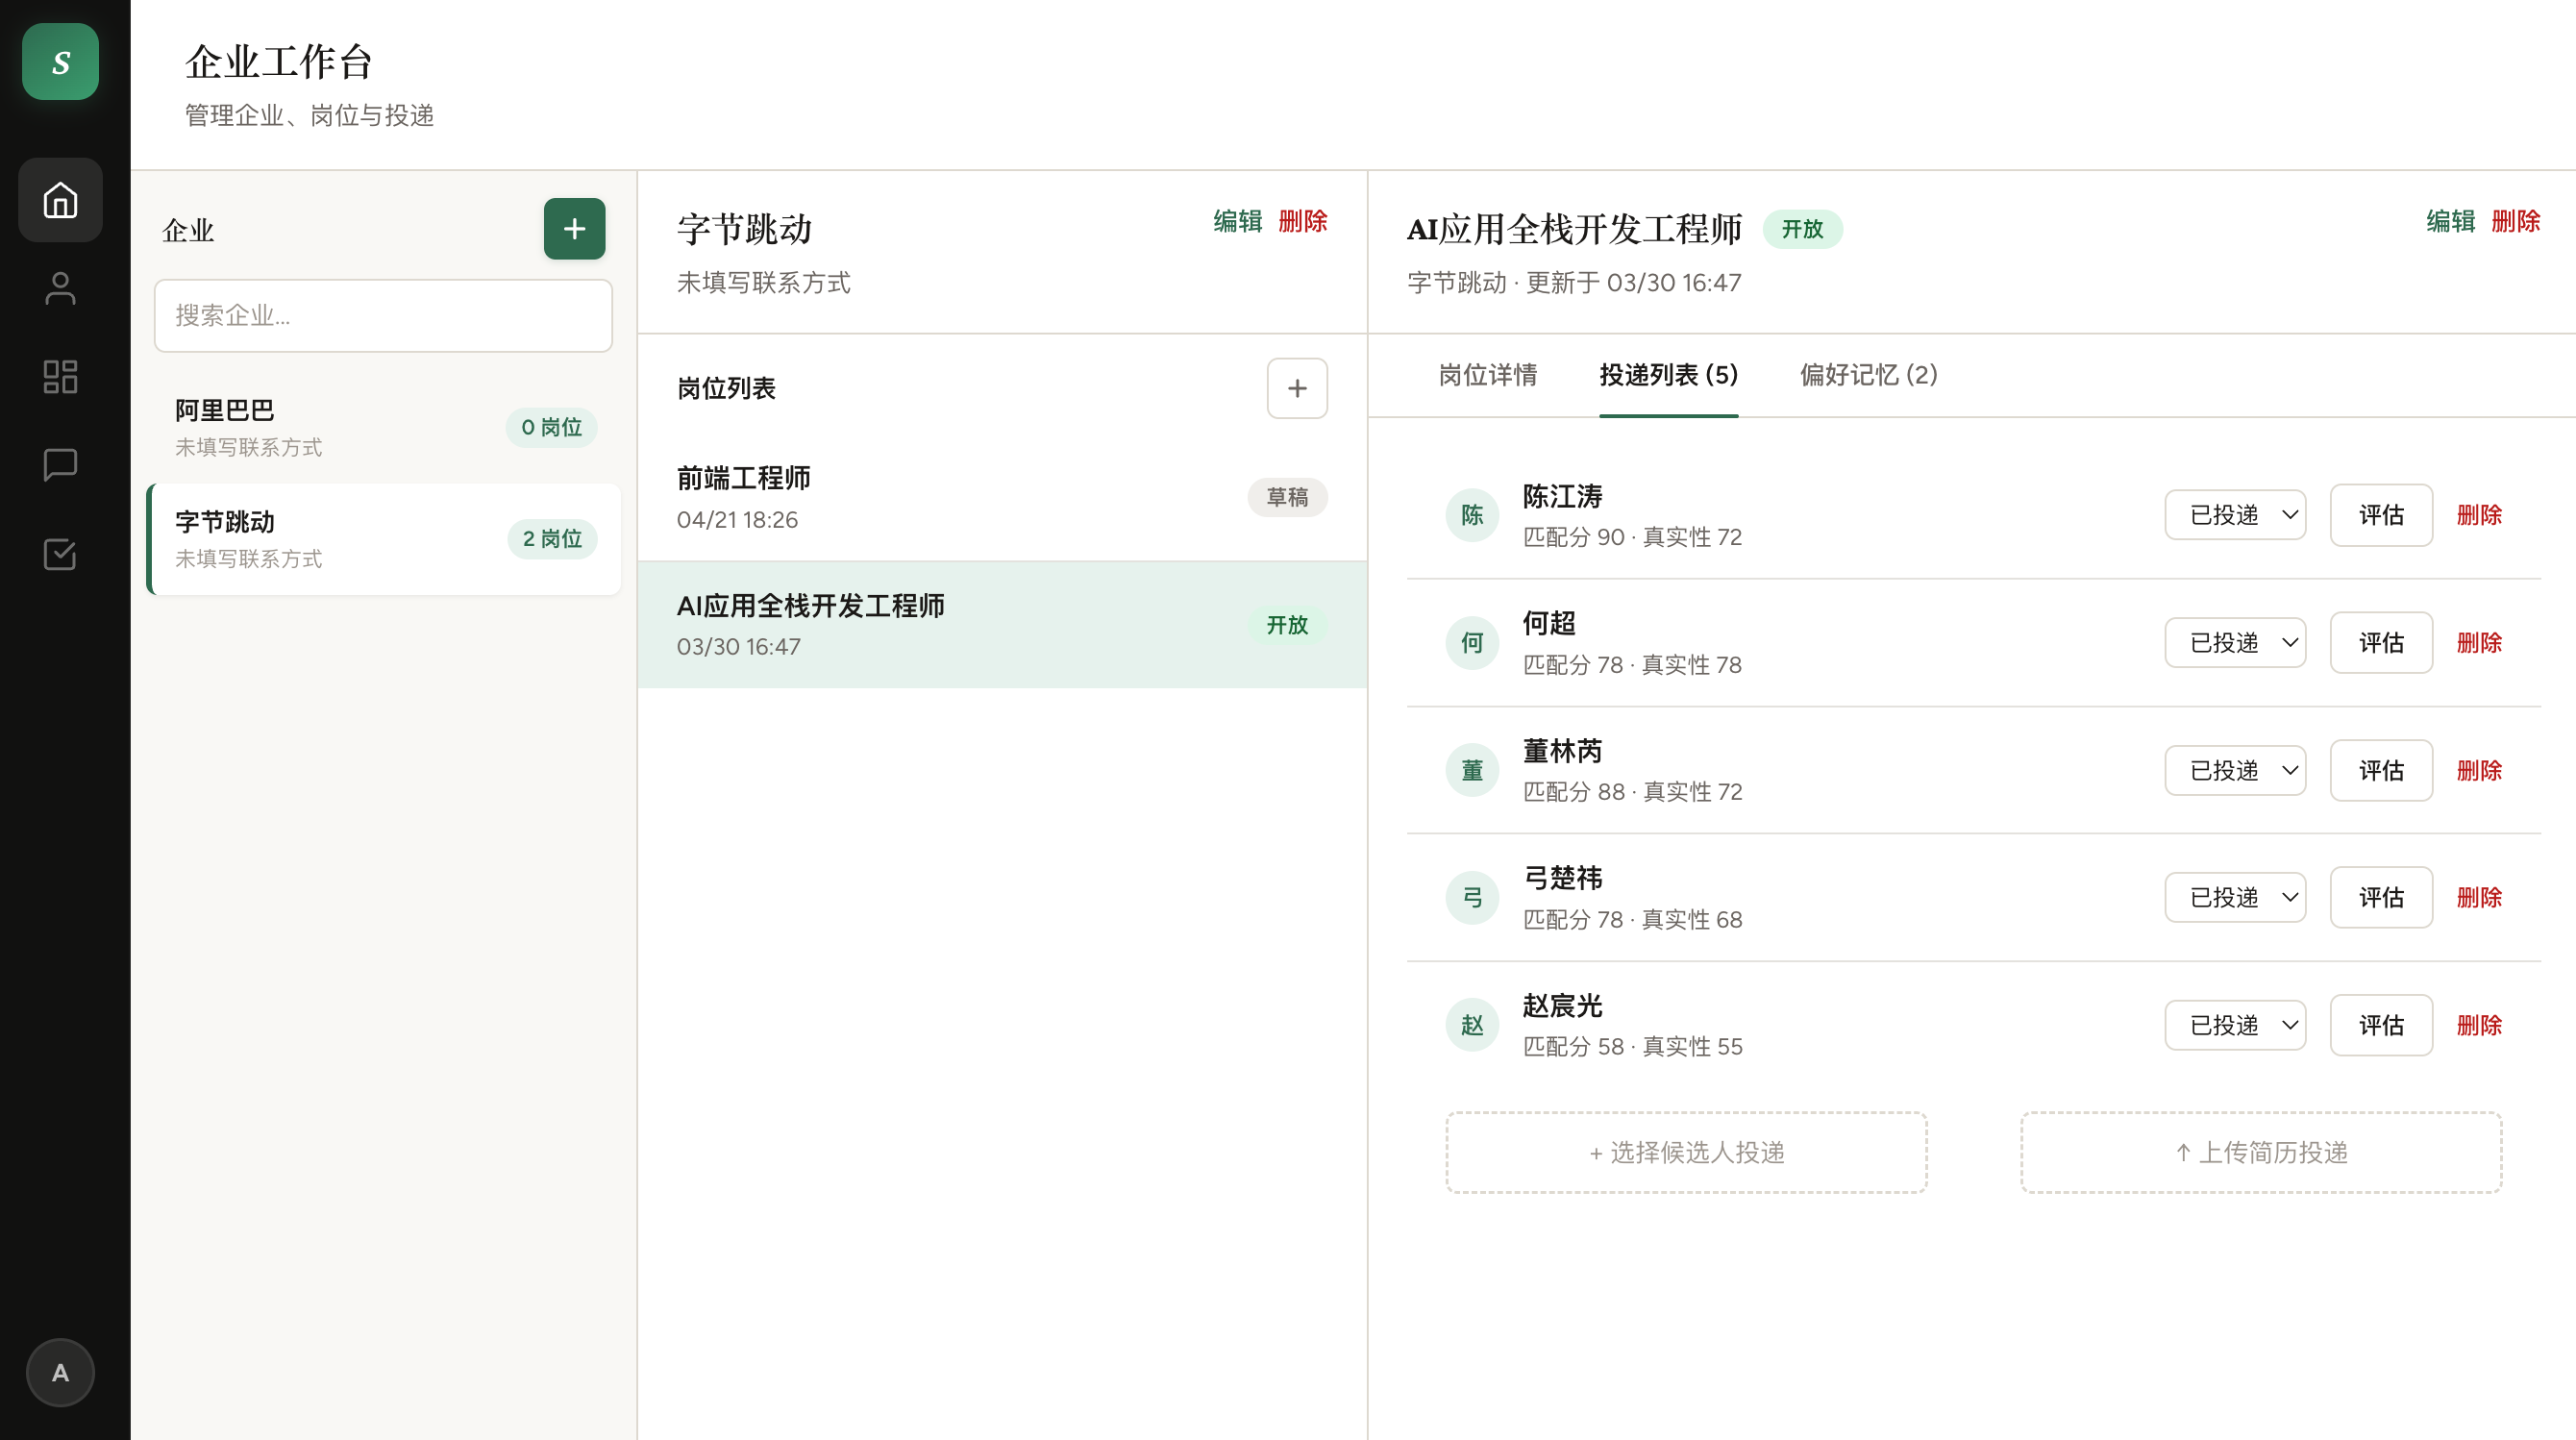
\includegraphics[width=0.96\textwidth]{media/enterprise.png}
\caption{企业与岗位工作台：三栏布局}
\label{fig:page-enterprise}
\end{figure}

企业与岗位管理页是\textbf{招聘流程的入口}，所有评估的上游数据都在此创建与维护。页面采用三栏式工作台：

\begin{itemize}[itemsep=2pt]
  \item \textbf{左栏 · 企业列表}：企业的搜索、新建、编辑、删除；
  \item \textbf{中栏 · 岗位列表}：进入企业后展示其下所有 JD，支持新建岗位与状态切换（草稿 / 开放 / 关闭）；
  \item \textbf{右栏 · 岗位详情}：以 Tab 形式分别展示岗位详情、投递列表与\textbf{偏好记忆}（由 Agent 自动沉淀的企业级与岗位级偏好，支持人工删除）。
\end{itemize}

这一页是后续所有评估的"上下文池"——后端记忆系统会持续向这里 upsert 偏好条目。

\subsection{候选人管理}

\begin{figure}[H]
\centering
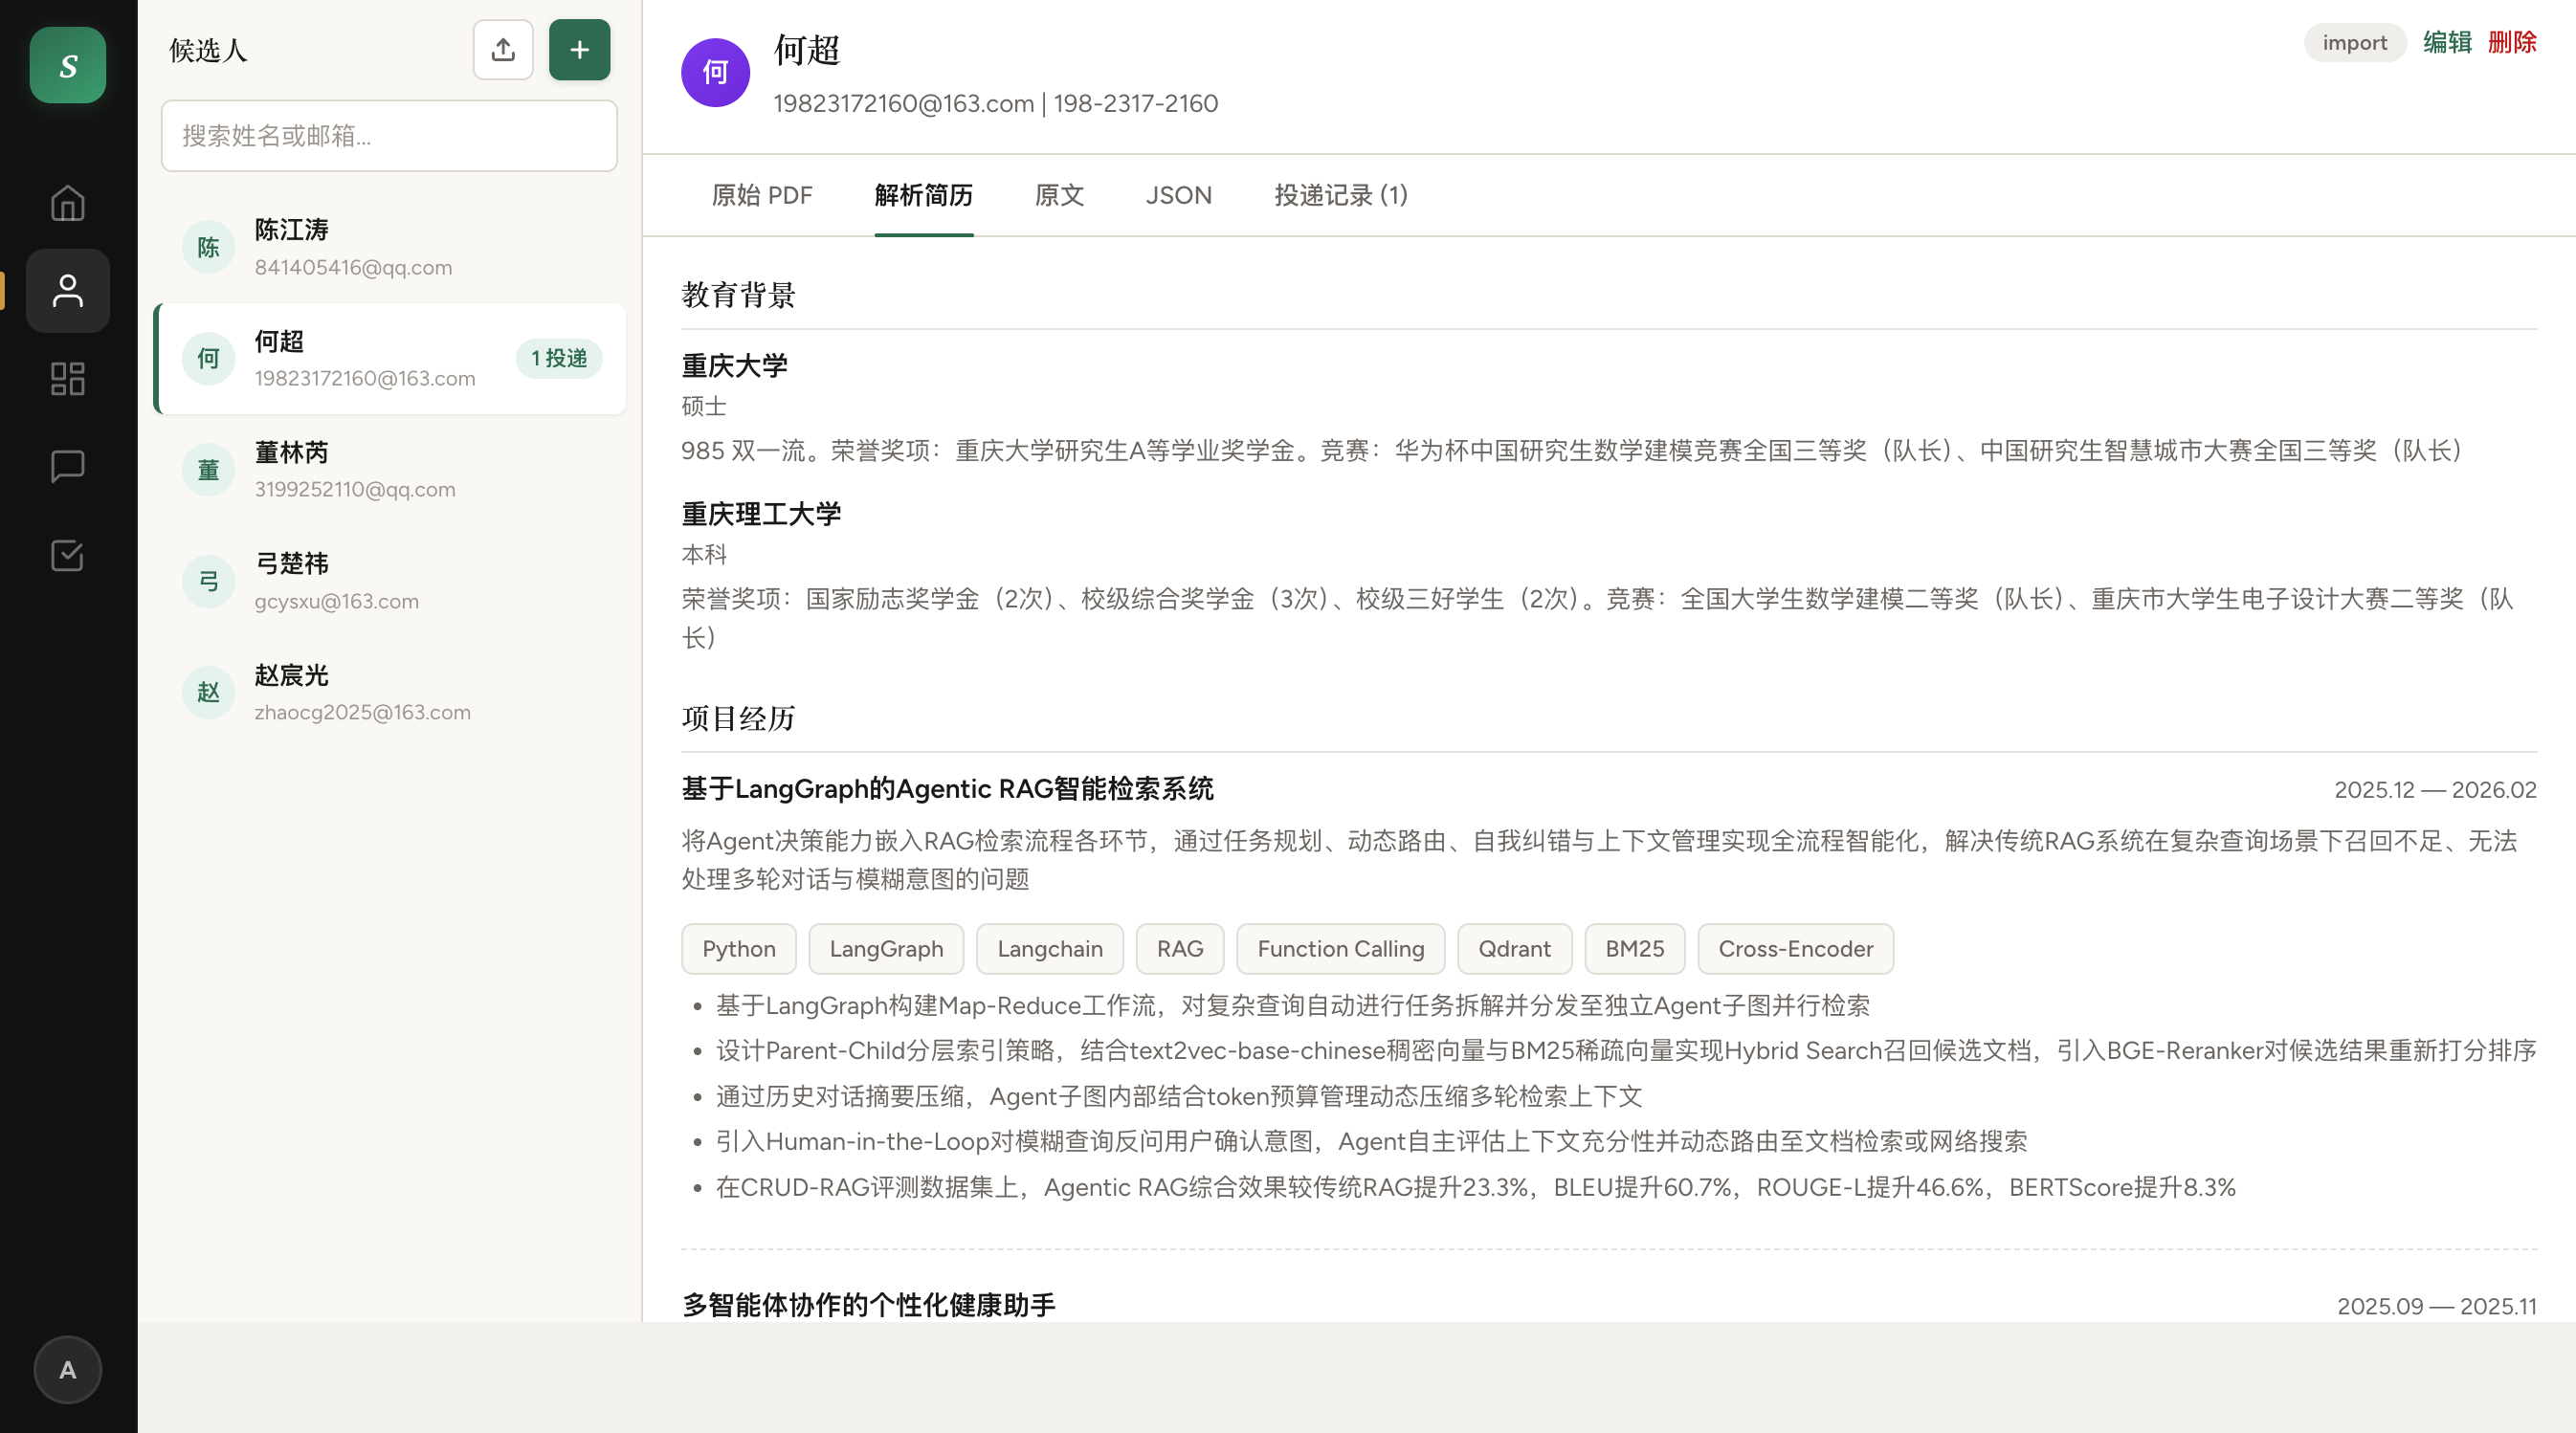
\includegraphics[width=0.96\textwidth]{media/candidate.png}
\caption{候选人库：简历的全生命周期管理}
\label{fig:page-candidate}
\end{figure}

候选人管理页负责把非结构化 PDF 简历转化为可检索、可复用的候选人 Profile。左栏为候选人列表（按姓名/邮箱搜索），右栏以多 Tab 展示候选人详情：原始 PDF（浏览器内嵌预览）、解析简历（结构化字段）、原文（纯文本）、JSON（完整 \texttt{parsed\_json}）、投递记录。上传 PDF 后自动启动 \texttt{parse\_status} 轮询（pending $\to$ parsing $\to$ completed / failed），无需手动刷新。该页的解析能力对应第~\ref{sec:exp}~章的 Qwen + CoT 模块，F1 由 66\% 提升到 78\%。

\subsection{批量化评估看板}

\begin{figure}[H]
\centering
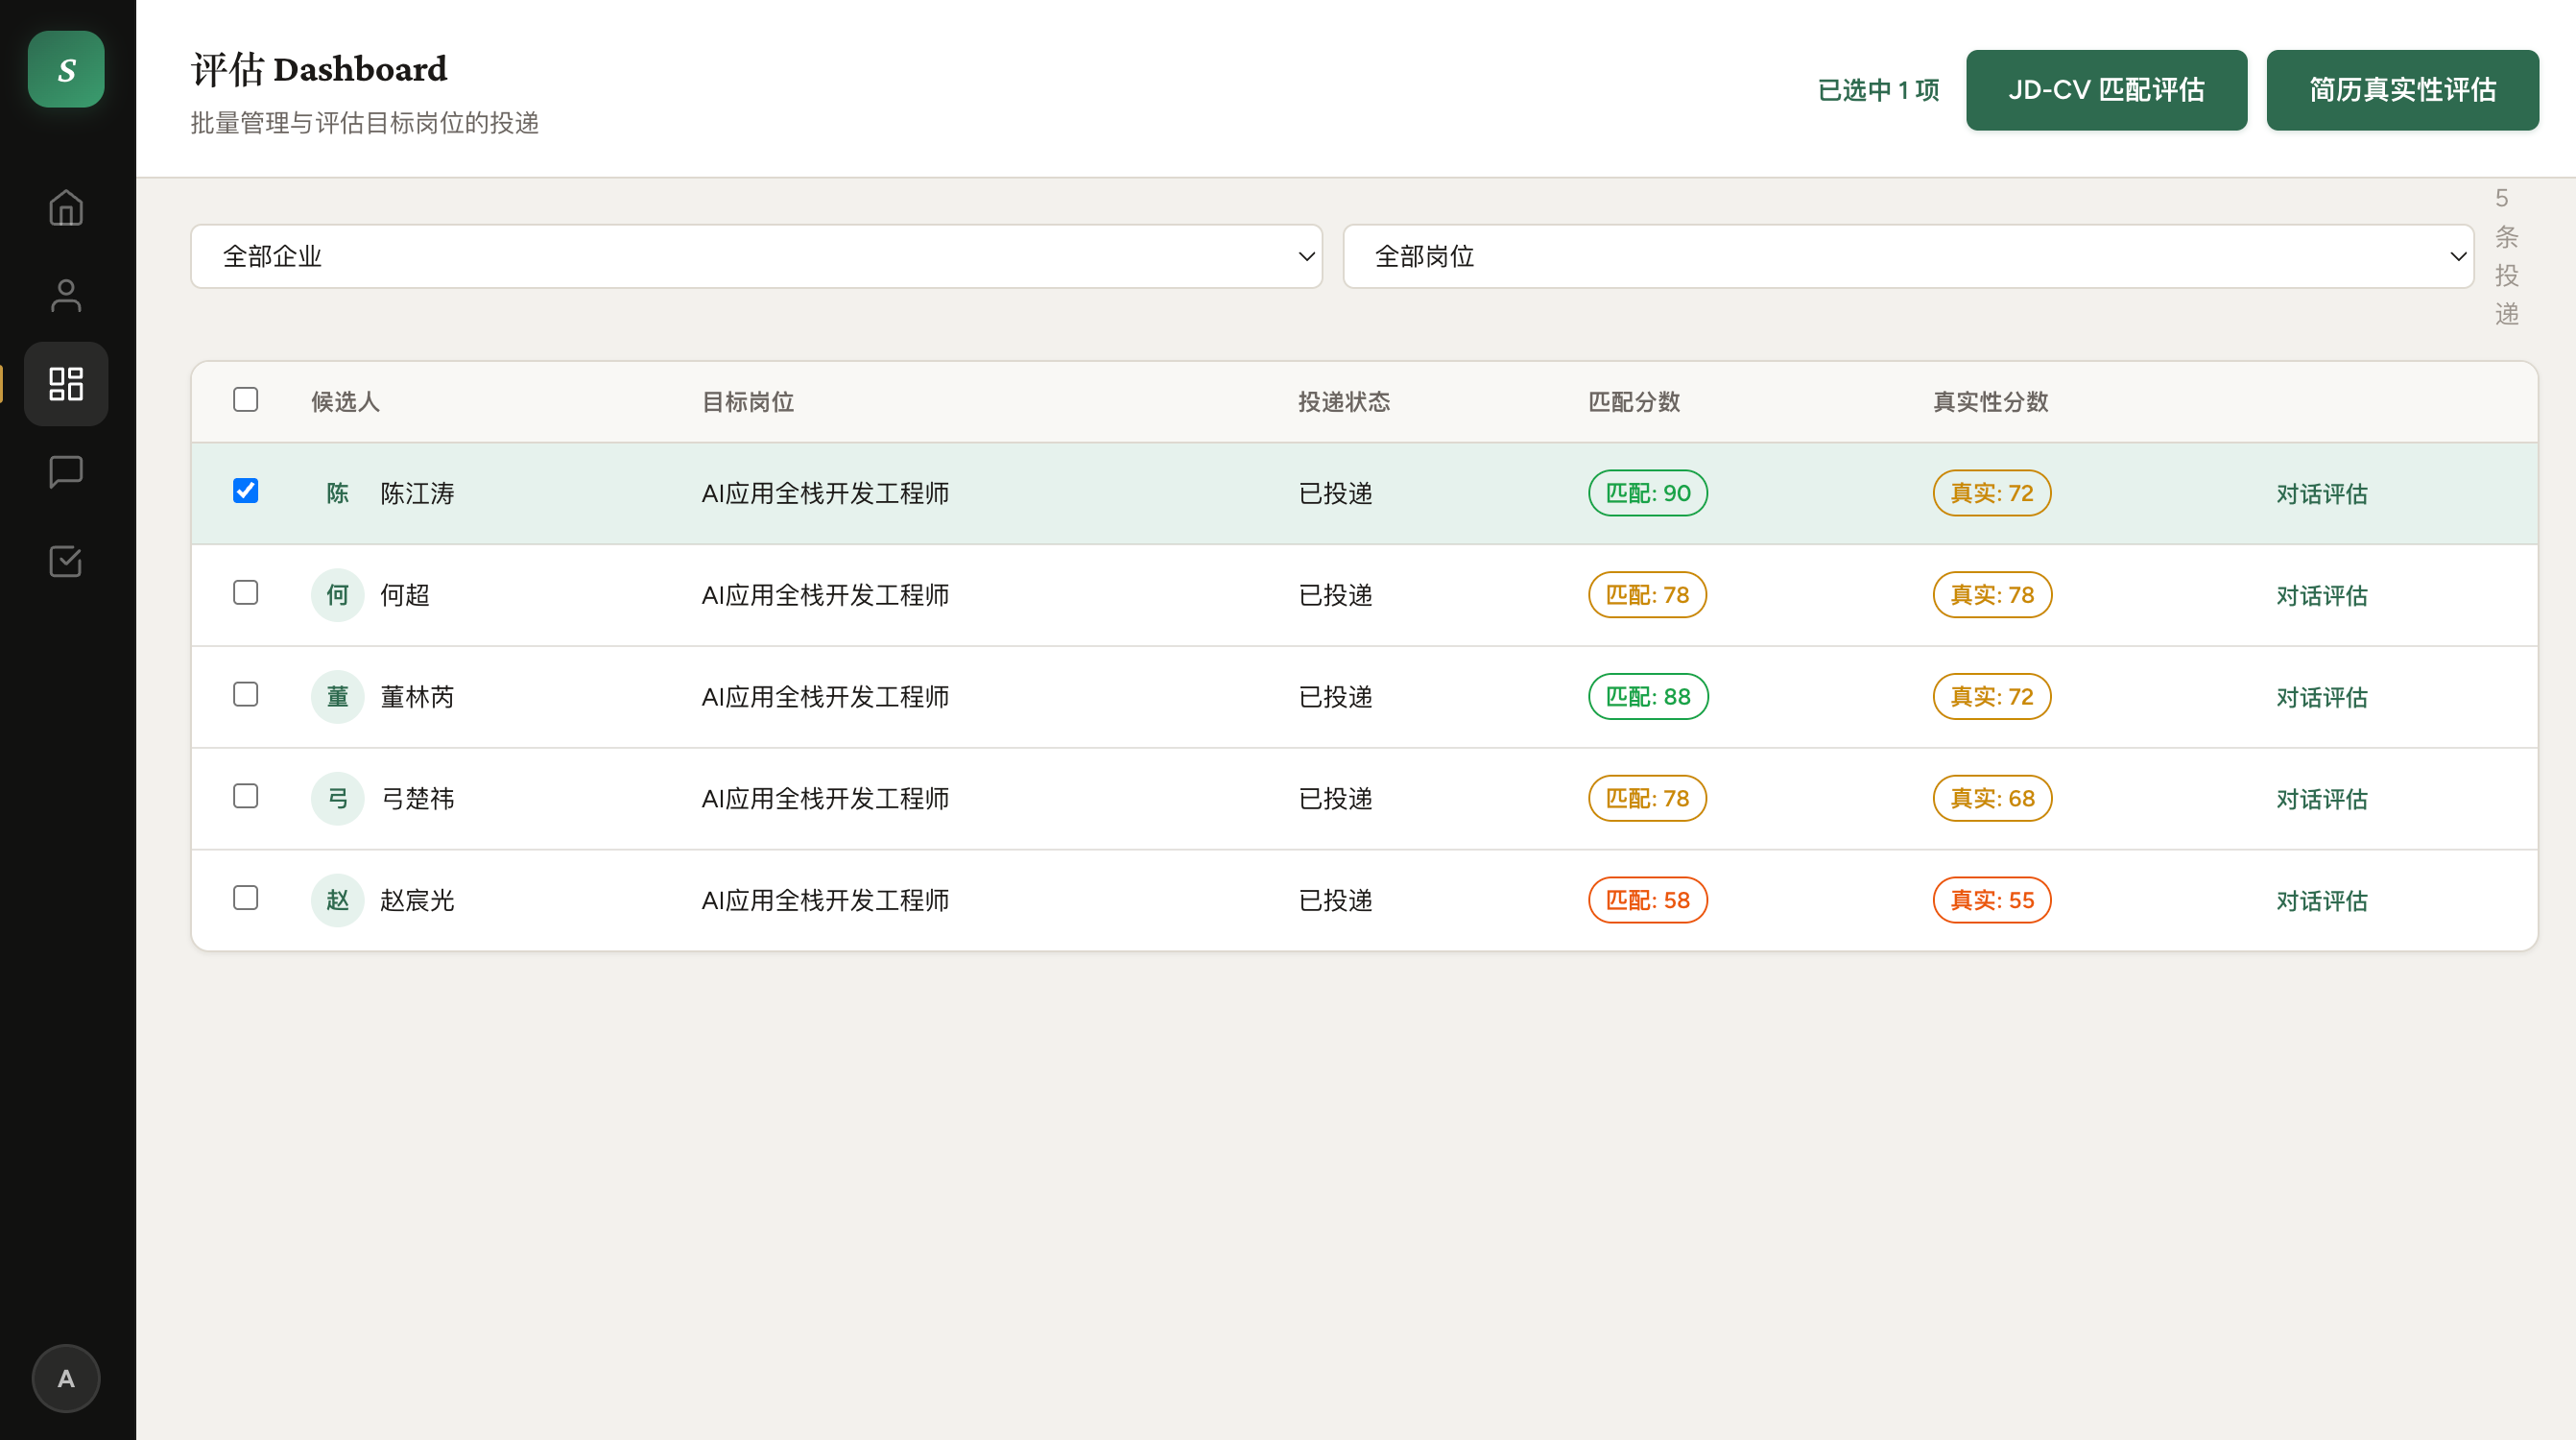
\includegraphics[width=0.96\textwidth]{media/dashboard.png}
\caption{批量化评估看板：双任务并列触发}
\label{fig:page-dashboard}
\end{figure}

批量化评估页是"流水线作业"形态：用户先按"企业 / JD"两级下拉过滤投递列表，再批量勾选目标投递；顶部并列两个批量任务按钮——\textbf{JD-CV 匹配评估}（5 维度：技能匹配、经验相关性、教育背景、行业契合度、综合潜力）与\textbf{简历真实性评估}（5 维度：时间线连贯性、职责合理性、成就可信度、信息完整性、一致性）。每行结果以双分数徽章呈现（匹配分 + 真实性分），按 80/60/40 分阈值自动染色（绿/黄/橙/红）；点击分数即可弹出评估报告 Modal，包含环形分数、等级徽章、维度条形图与优势/不足/风险点列表。这一页的目标是"快"——给出量化结论让 HR 先压缩漏斗，深度判断交给第~5.5~节。

\subsection{深度评估 Agent（重点）}

\begin{figure}[H]
\centering
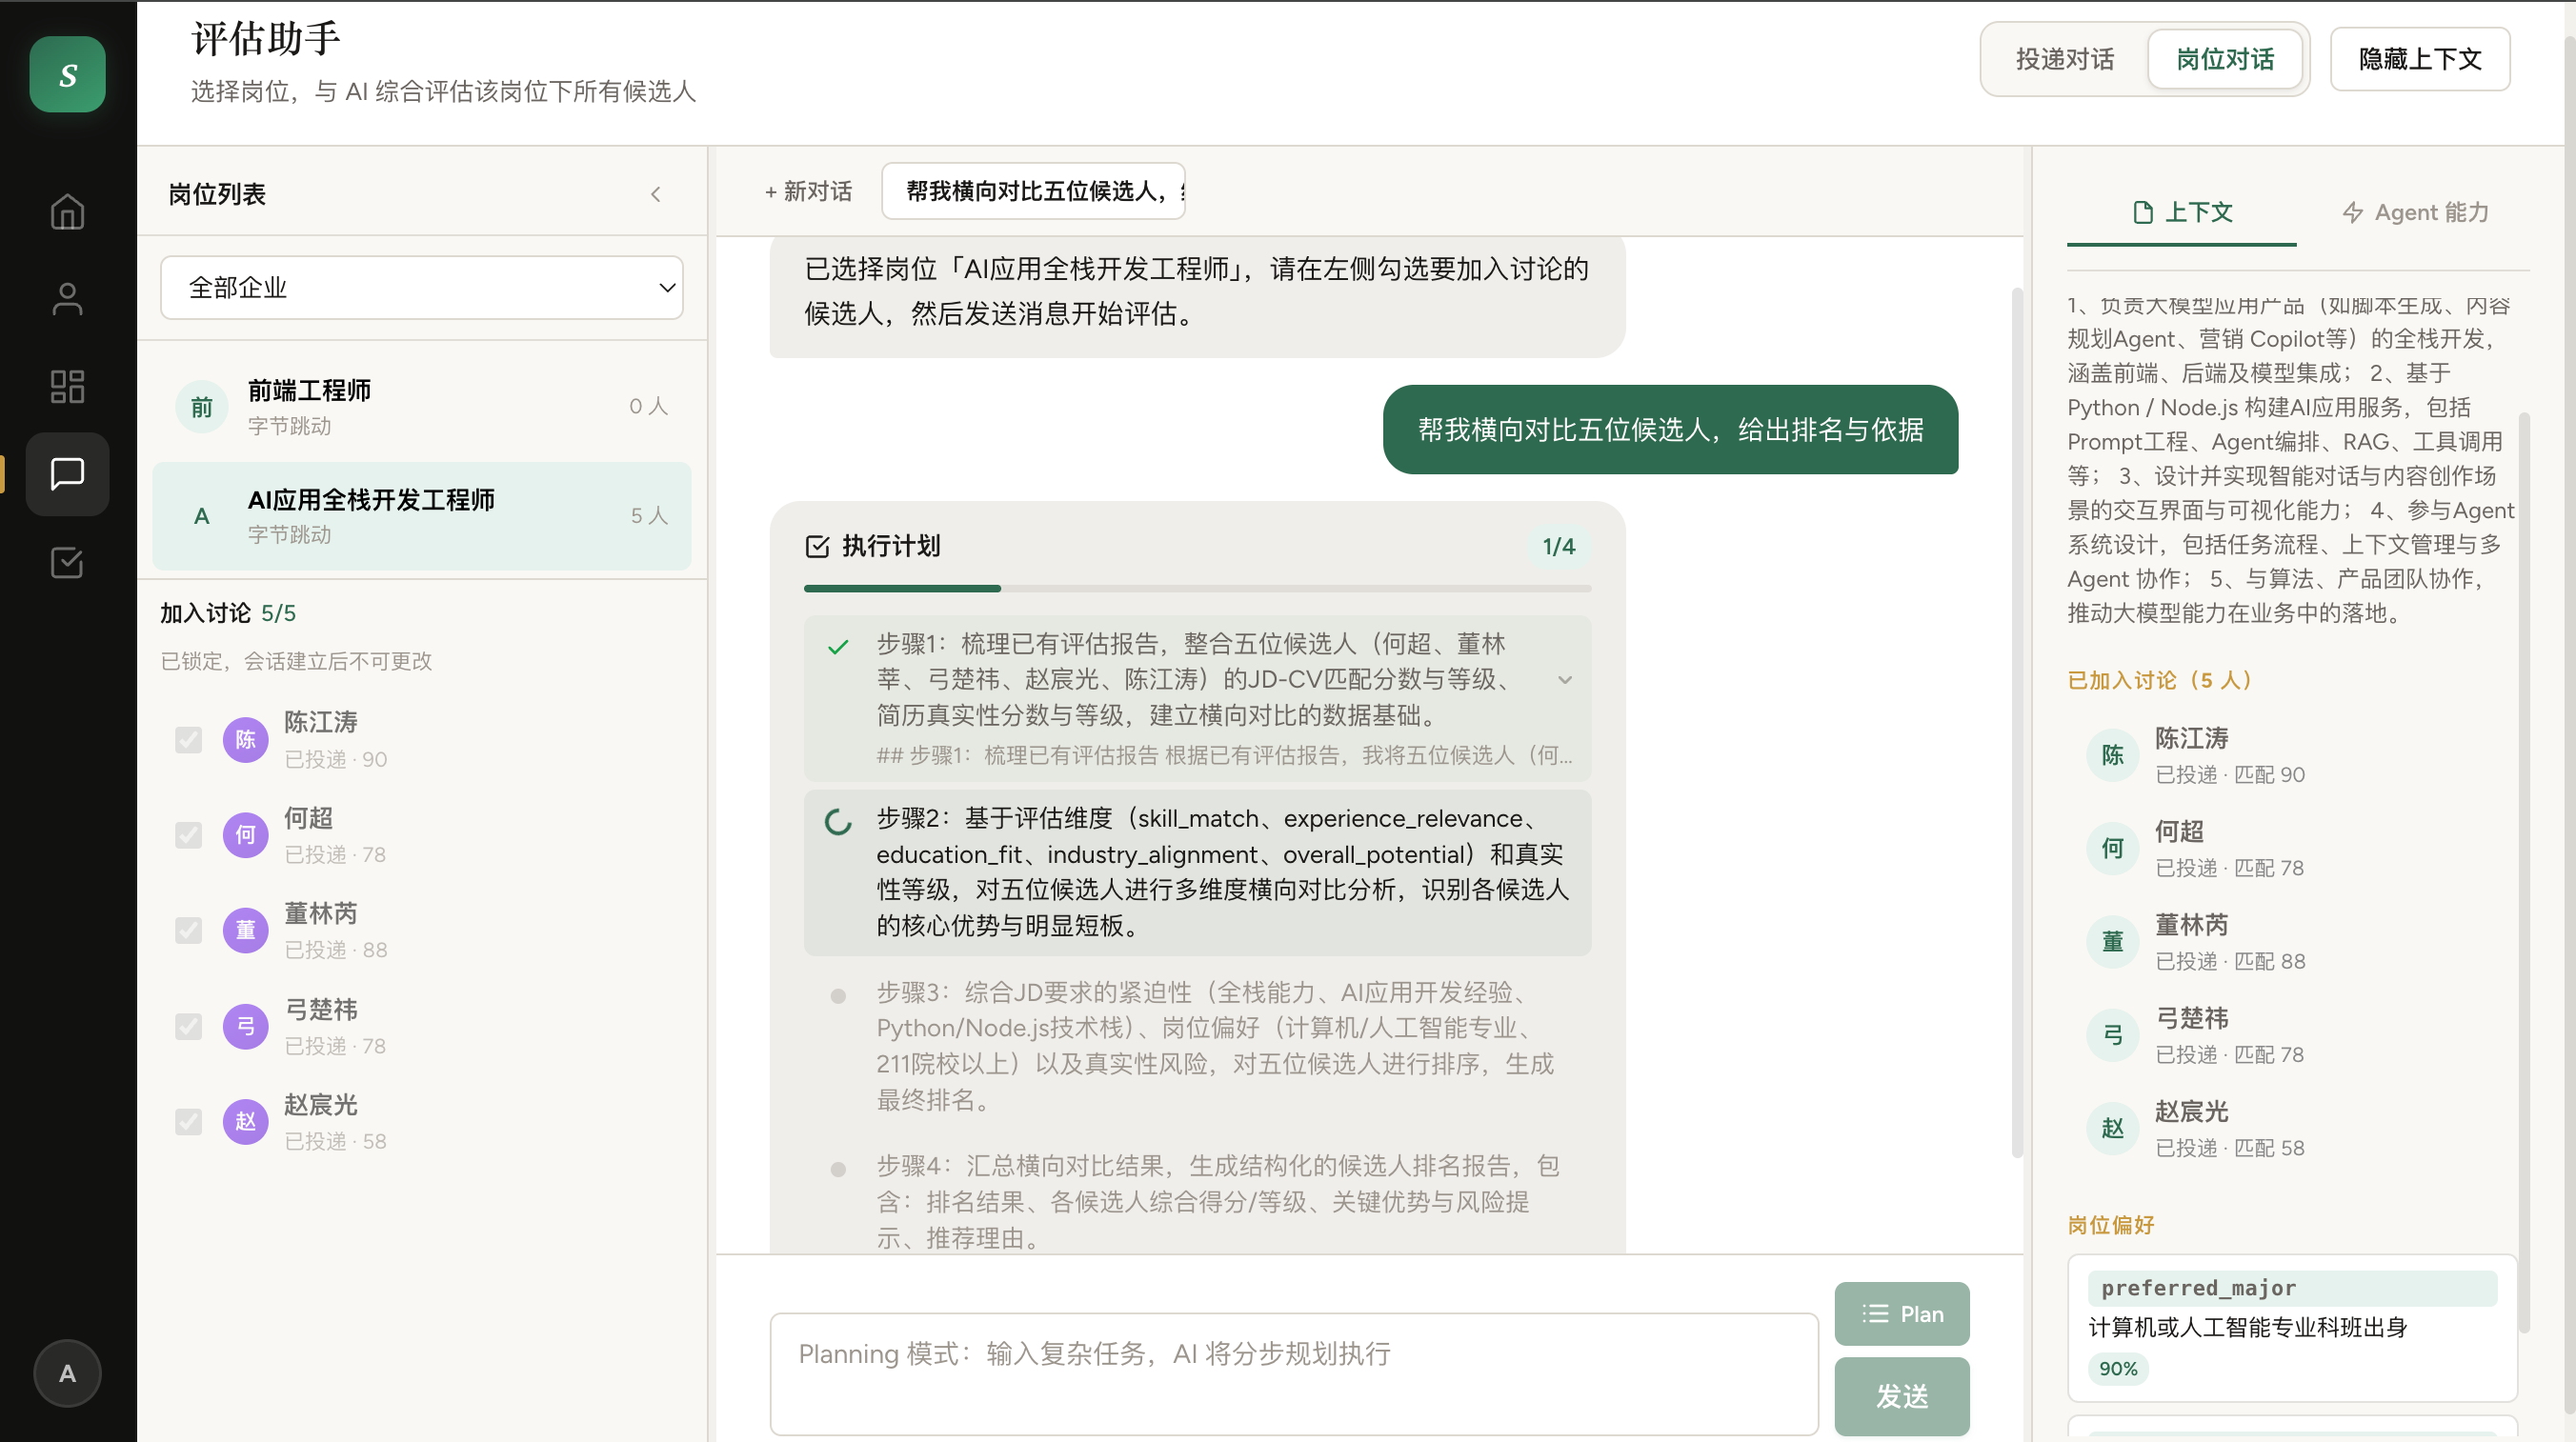
\includegraphics[width=0.96\textwidth]{media/assistant.png}
\caption{深度评估 Agent：三栏对话界面与 Plan 可视化}
\label{fig:page-assistant}
\end{figure}

深度评估 Agent 是项目的\textbf{核心交付物}：把"打分流水线"升级为"会调工具、有记忆、能规划"的 Agent，让 HR 能像和资深面试官对话一样深挖每一份候选人或每一个岗位。

\subsubsection{整体布局与两种对话模式}

页面顶部为模式切换条，主体为三栏布局——左栏为投递/岗位列表（含候选人勾选区），中栏为多轮对话区（含会话 Tab 与消息流），右栏为上下文与能力面板（Context Tab / Capabilities Tab）。两种对话模式的差异见表~\ref{tab:dialog-mode}。

\begin{table}[H]
\centering
\renewcommand{\arraystretch}{1.3}
\caption{深度评估 Agent 的两种对话模式}
\label{tab:dialog-mode}
{\small
\begin{tabular}{L{2.4cm} L{3.0cm} L{3.4cm} L{3.4cm}}
\toprule
\textbf{模式} & \textbf{触发条件} & \textbf{上下文范围} & \textbf{适用场景} \\
\midrule
\texttt{application} 投递对话 & 选中一条投递记录 & 单候选人 $\times$ 单 JD & 单点深挖：一个人到底合不合适 \\
\texttt{jd} 岗位对话 & 选中 JD + 勾选若干候选人 & 一个 JD $\times$ N 个候选人 & 横向比较：在 N 个候选人里选谁 \\
\bottomrule
\end{tabular}
}
\end{table}

\subsubsection{会话管理：持久化与断流恢复}

这是该页工程含量最高的部分。系统为每条投递 / 每个 JD 都维护独立的历史会话列表（\texttt{listChatSessions}），支持多 Tab 切换、新建、删除。跨页面持久化通过 \texttt{sessionStorage} 同时缓存 \texttt{assess\_chat\_nav}（当前模式 / 选中 ID / \texttt{sessionId} / \texttt{runId} / \texttt{lastSeq}）和 \texttt{assess\_chat\_msgs}（完整消息列表），即使用户跳到别的页面再回来，对话状态、Plan 步骤、已收 token 都能原样恢复。如果用户在 Agent 还在流式输出时离开页面，回来后会自动调用 \texttt{resumeAgentStream(runId, lastSeq)} 从断点续传，恢复失败则 fallback 到 \texttt{listChatMessages} 重新拉取历史。

\subsubsection{SSE 七类流式事件渲染}

后端通过 SSE 推送七类事件，前端用 \texttt{chatWithAgentStream} 的 \texttt{ChatStreamHandlers} 分别接管（表~\ref{tab:sse-events}）。

\begin{table}[H]
\centering
\renewcommand{\arraystretch}{1.3}
\caption{SSE 事件类型与前端反应}
\label{tab:sse-events}
\begin{tabular}{L{3.0cm} L{8.6cm}}
\toprule
\textbf{事件} & \textbf{前端反应} \\
\midrule
\texttt{onSession} & 拿到 \texttt{session\_id} / \texttt{run\_id}，刷新会话 Tab \\
\texttt{onEventSeq} & 维护 \texttt{lastSeqRef}，用于断流续传定位 \\
\texttt{onThinking} & 渲染顶部"正在制定执行计划… / 执行步骤 3/7…"进度条 \\
\texttt{onPlan} & 把 plan 数组渲染为 \textbf{PlanTracker} 组件 \\
\texttt{onStepDone} & 把对应步骤标记为完成，下一步置为 executing \\
\texttt{onReplan} & 保留已 done 的步骤，后续步骤替换为新计划 \\
\texttt{onToken} & 把 token 增量 append 到 Markdown 气泡 \\
\texttt{onDone / onError} & 收尾、停止 spinner、错误兜底 \\
\bottomrule
\end{tabular}
\end{table}

\subsubsection{Planning 模式可视化}

输入框右侧的 Plan 切换按钮控制后端 \texttt{use\_planning} 字段。开启后，用户消息送出后立即出现一条 \textbf{PlanTracker} 气泡（占位、空步骤）；收到 \texttt{onPlan} 后渲染步骤列表，第一步置为 executing（带 spinner），其余为 pending（灰点）；每收到 \texttt{onStepDone} 即将该步打勾并展示一段 \texttt{result\_preview}，下一步自动接力；\texttt{onReplan} 则保留已完成步骤，后续重排——这正是第~\ref{sec:agent}~章中 Plan-and-Execute 范式的前端可视化。最终 Markdown 报告以新气泡追加在 PlanTracker 之后。

\subsubsection{右栏：上下文与能力面板}

右栏的 \textbf{Context Tab} 根据当前模式动态展示：投递模式下提供候选人卡 + 简历摘要 + 岗位信息 + 投递状态 + 历史评估报告 + 企业/岗位偏好；岗位模式下展示岗位信息卡 + "已加入讨论"候选人列表 + 偏好。\textbf{Capabilities Tab} 通过 \texttt{getAgentCapabilities} 拉取后端实际注册的能力清单，分技能模块（Skills）、内置工具（Tools）与 MCP 服务三类透明展示，让 HR 知道 AI 此刻能调哪些外部能力，不再是黑盒。

\subsubsection{与 Agent 三要素的呼应}

把 5.5.1--5.5.5 串起来看，正好对应第~\ref{sec:agent}~章给出的"为什么必须是 Agent"的三要素（表~\ref{tab:agent-elements-page}）。

\begin{table}[H]
\centering
\renewcommand{\arraystretch}{1.3}
\caption{深度评估 Agent 页面对 Function Calling / Memory / Planning 的可见体现}
\label{tab:agent-elements-page}
\begin{tabular}{L{3.2cm} L{8.4cm}}
\toprule
\textbf{Agent 要素} & \textbf{在该页的具体体现} \\
\midrule
Function Calling & Capabilities Tab 中的 Tools / Skills / MCP；Context 里的简历、JD、KG 偏好都是工具产物 \\
Memory & 会话级 Tab 条 + sessionStorage + 断流恢复；Context Tab 中的"企业 / 岗位偏好"是长期记忆 \\
Planning & Plan 切换按钮 + PlanTracker + Replan 事件，把 LangGraph 的多步规划与重规划完整可视化 \\
\bottomrule
\end{tabular}
\end{table}

这也是该页与第 5.4 节"批量评估"最本质的区别——\textbf{批量评估只能给一个分数，深度评估 Agent 能讲清楚"为什么是这个分数"，并支持继续追问}。

\subsection{Eval 系统}

\begin{figure}[H]
\centering
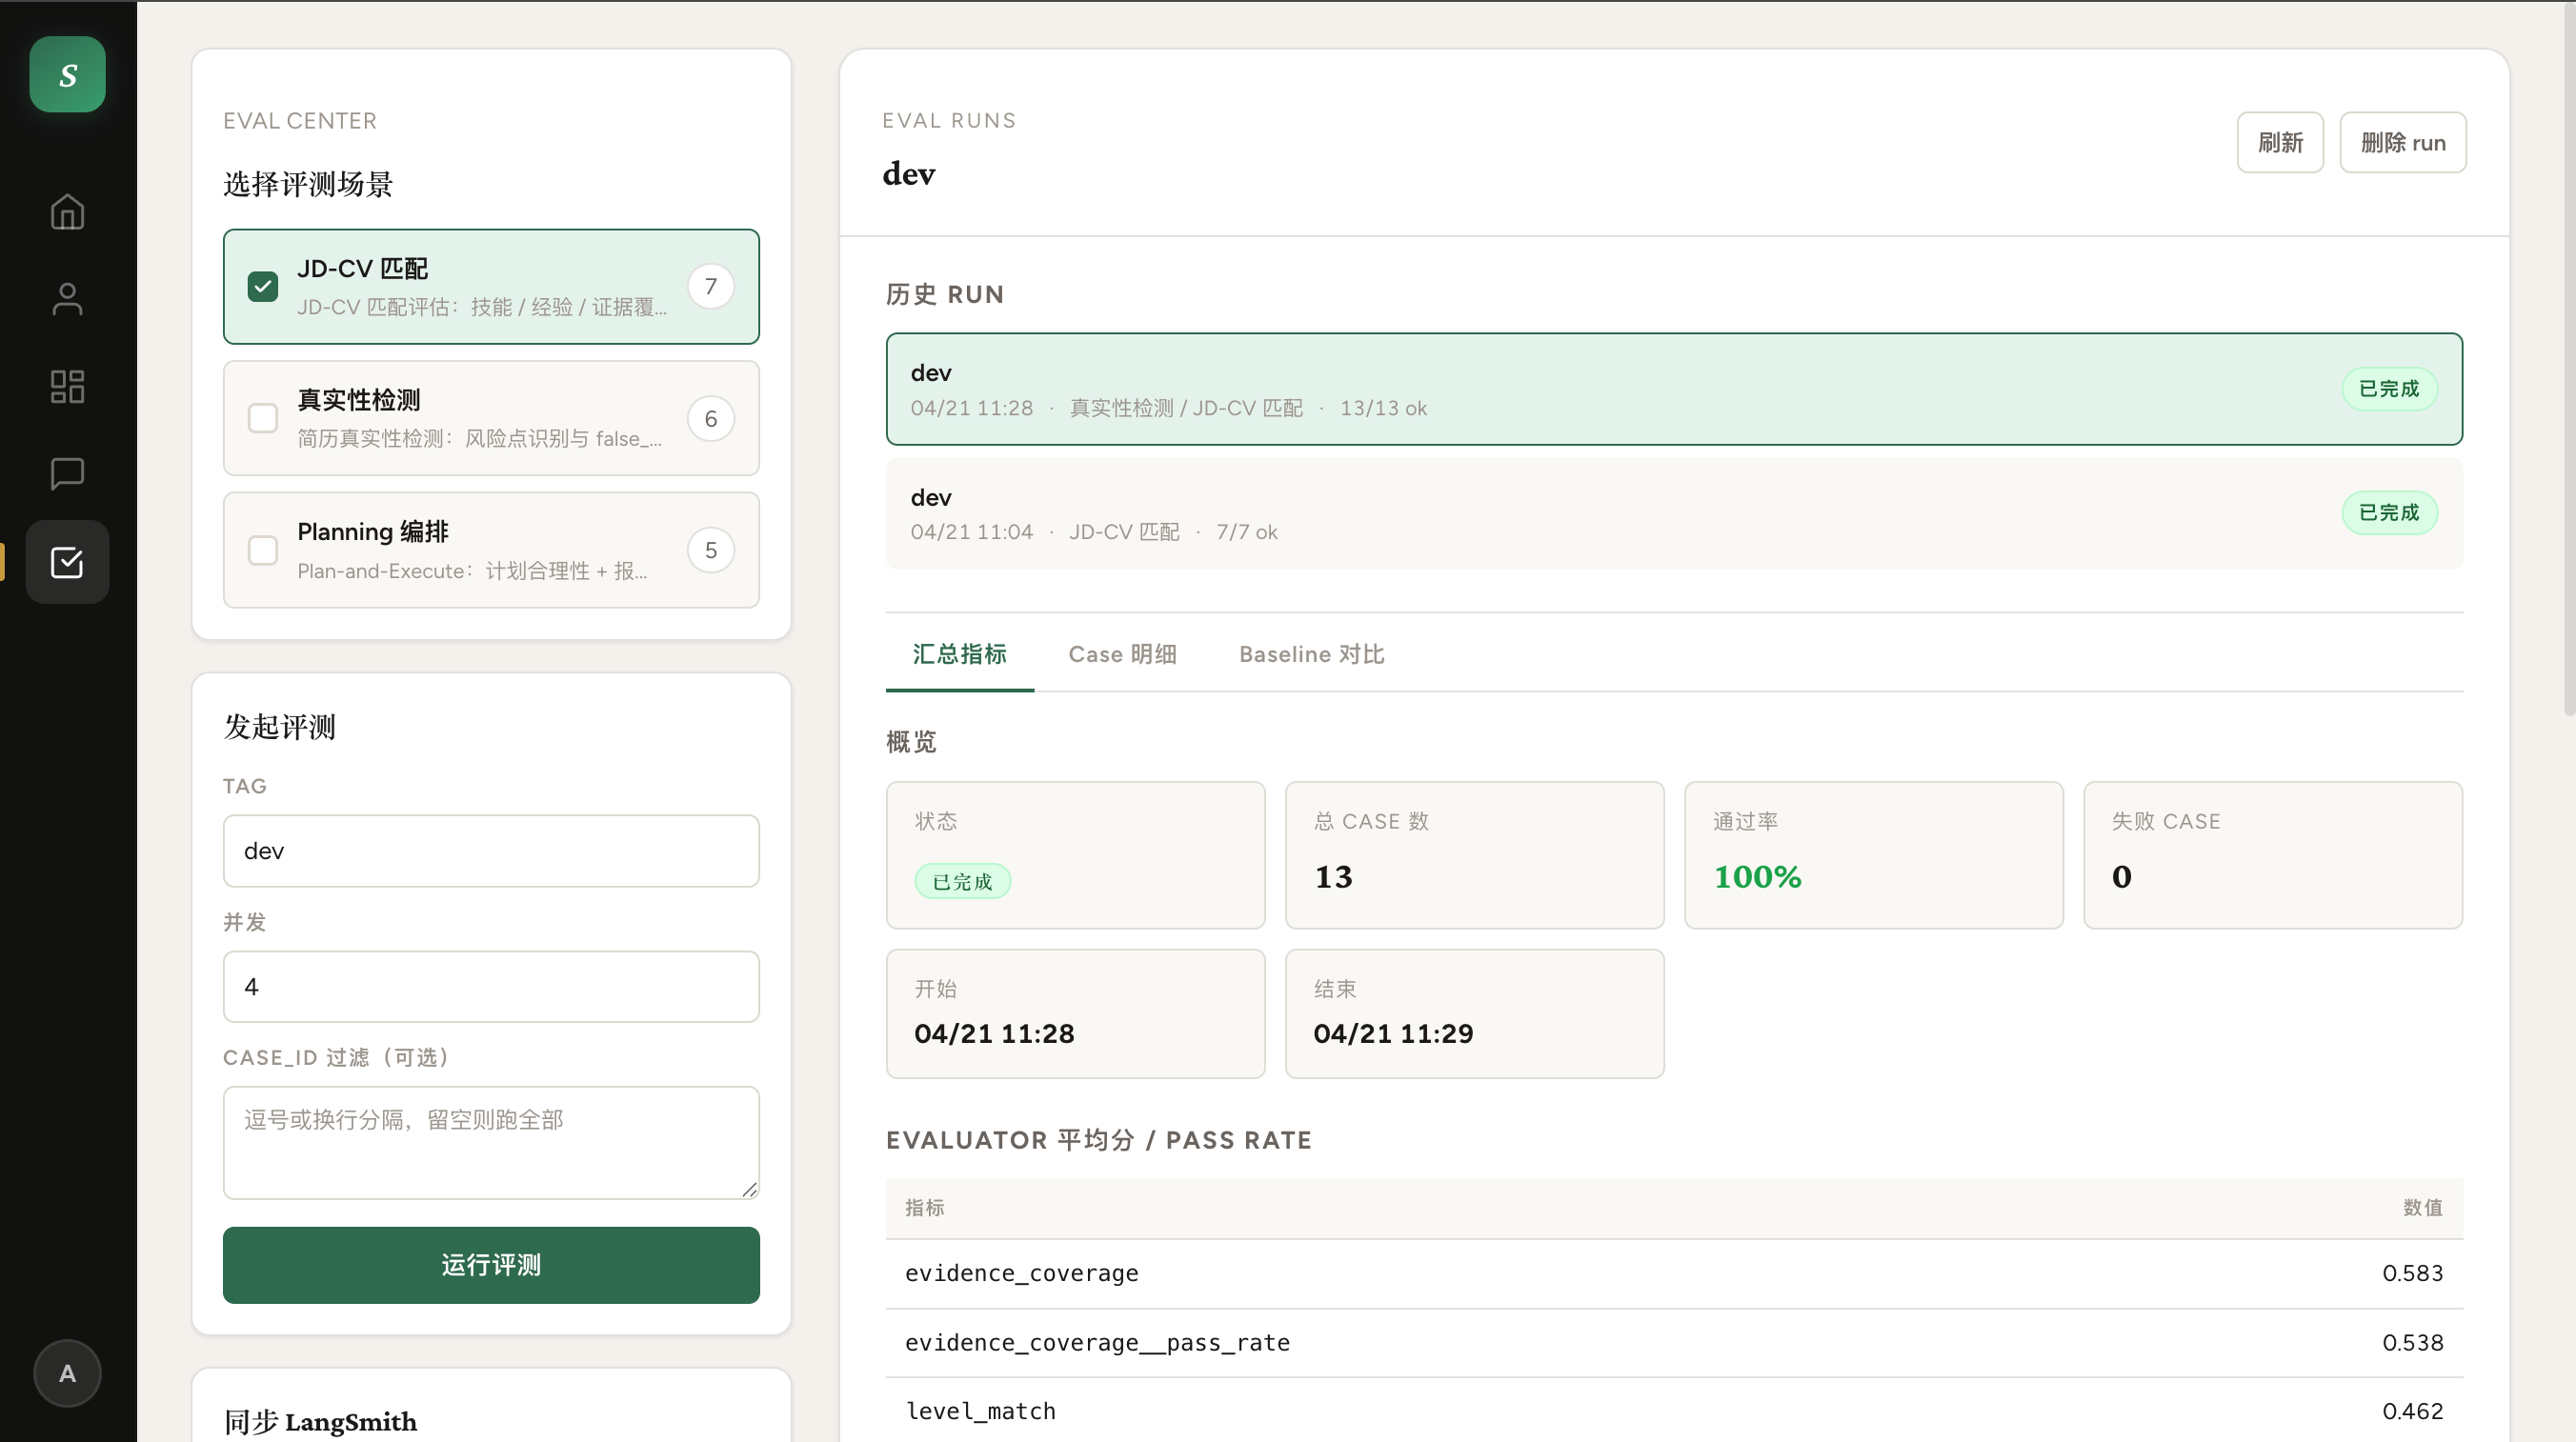
\includegraphics[width=0.96\textwidth]{media/eval.png}
\caption{Eval 系统：离线评测中心}
\label{fig:page-eval}
\end{figure}

Eval 系统是面向开发者的离线评测工作台，不在业务流上，专门用于回归 Agent 质量。三大评测场景与后端 \texttt{evaluators} 对齐：\texttt{jd\_cv\_match}、\texttt{authenticity}、\texttt{planning}。主要功能区包括：

\begin{itemize}[itemsep=2pt]
  \item \textbf{创建 Run}：勾选场景、设置 tag（如 \texttt{dev} / \texttt{prod}）、并发数与 case 过滤器，一键 \texttt{createEvalRun}；
  \item \textbf{Run 列表}：所有历史 run 状态徽章（排队 / 运行 / 完成 / 失败），运行中的 run 自动 4 秒轮询刷新进度；
  \item \textbf{详情面板（三 Tab）}：Summary 展示 \texttt{aggregate\_scores}（通用指标）与 \texttt{business\_metrics}（场景业务指标）；Cases 列出每条 case 的输入 / 期望 / 实际输出 / evaluator 子分；Compare 在选定 baseline run 后做 \texttt{compareEvalRuns}，逐指标显示 $\Delta$ 与方向（区分"越大越好"/"越小越好"）；
  \item \textbf{数据集同步}：\texttt{syncEvalDataset} 一键把当前评测集同步到 LangSmith dataset。
\end{itemize}

这一页让"每一次模型 / Prompt / Skill 的改动"都能被定量回归，是 Agent 项目能持续迭代的工程基石。

% ==================================================
% 第六章 结论与展望
% ==================================================
\section{结论与展望}\label{sec:conclusion}

\subsection{核心结论}

围绕招聘行业"关键词匹配失效、简历过度包装、能力评估粗糙、信息碎片化"四类核心痛点，本项目以 ScoutAgent 为载体给出了一套从需求到落地的完整方案。三项关键算法在与基线的对照实验中均取得显著提升：

\begin{itemize}[itemsep=2pt]
  \item \textbf{结构化信息抽取}：F1 由 66\%（Zero-shot）提升至 78\%（Qwen + CoT），简历评测样本量 5{,}960；
  \item \textbf{GraphRAG 匹配增强}：JD/CV 二分类准确率由 74.3\%（纯 LLM）提升至 85.2\%（LLM + KG），相对提升约 10.9 个百分点；图谱多跳推荐在 Hit@5 与 MRR 上同步优于共现与词频基线；
  \item \textbf{过度包装检测}：Pairwise Accuracy 由 73.5\%（Zero-shot）提升至 88.5\%（SFT + DPO），F1 同步从 67.8\% 提升至 80.5\%。
\end{itemize}

工程上，本项目以 LangGraph 为编排核心同时落地了 ReAct 与 Plan-and-Execute 双范式，统一组合 Tools / Skills / MCP 三层工具，并通过 Redis Checkpointer 与 PostgreSQL 偏好库实现两层记忆体系。前端则把 Function Calling、Memory、Planning 三要素以 Capabilities Tab、会话恢复与 PlanTracker 三种形态可视化呈现给 HR，使 Agent 不再是黑盒。

\subsection{局限与未来工作}

当前系统仍存在若干局限，对应几个明确的后续方向：

\begin{enumerate}[itemsep=3pt]
  \item \textbf{DPO 偏好闭环}：当前 DPO 数据由半自动管道合成，未来可以从 HR 实际反馈中持续采集偏好对，形成线上闭环；
  \item \textbf{岗位维度综合决策 Agent}：当前评估仍以单投递为粒度，未来可在岗位池上做相对排序与团队互补性分析；
  \item \textbf{跨企业偏好迁移}：当前偏好在企业级与岗位级两层 scope 内沉淀，未来可探索跨行业、跨岗位的偏好迁移机制；
  \item \textbf{多智能体代码评测}：未来可在 Sandbox 环境中引入代码执行评测 Agent，对候选人提交的代码片段做运行验证与过程评分，进一步增强能力评估的可量化程度。
\end{enumerate}

\vspace{1.2cm}
\begin{center}
\textit{——— 报告完 ———}
\end{center}

\end{document}
